\section{Yako} \label{yako}
     The implementation of the project is divided into two parts. On one hand, a back-end, where the orchestrator operates, where logic and computation take place. On the other hand, the front-end, a client that acts as a gateway to interact with all the computational resources available on the server side. A detailed description of all the fractions that comprises the project will be presented in the following sections.
    
    \begin{figure}[H]
        \centering
        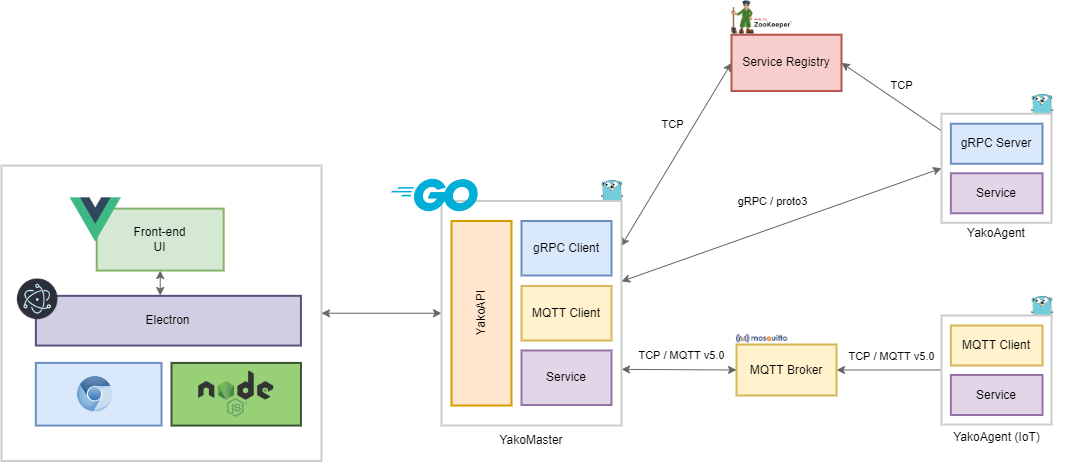
\includegraphics[width=\linewidth]{Backend/Simple Architecture.png}
        \caption{Yako platform simple architecture: (left) front-end application (right) orchestrator and services}
        \label{fig:simple_architecture}
    \end{figure}
    
    Figure \ref{fig:simple_architecture} represents the internal interconnection of the different components of the platform. An example of a more complex and extended system will be described at the end of this chapter on figure \ref{fig:complex_architecture}.
 
    \subsection{Back-end} \label{section:backend}
    \subsubsection{Architecture}
        Depending on the specific needs for a cluster, the architecture and internal structure might vary. However, as a general guideline, a computation cluster is generally comprised of computational nodes. As stated in the objective section \ref{objective}, the project aims to address heterogeneous environments, which translates into a context where different types of devices co-exist. Indifferently of the level of heterogeneity these are, in the Yako platform, all devices fall into three main categories which will be introduced in the next subsections. These are the YakoMaster, the YakoAgent and the YakoAgent (IoT).
        
        The platform currently only supports Linux based YakoAgents. Other types of OS are expected to be accepted in the future, this is discussed in the Future work section \ref{future_work}. 
        
    \subsubsection{Service Registry}
        The service registry, outlined in red in figure \ref{fig:simple_architecture}, is one of the core component of the complete system. It leverages this feature from Apache Zookeeper's distributed system coordination and metadata storage. It is a widely used pattern in real world production environments, like Netflix's infrastructure \cite{netflix_technology_blog_netflix_2017}, Kubernetes \cite{cloud_native_computing_foundation_operating_nodate}, to name a few.
        The service registry is best suited for environments where the number of services instances and their locations changes dynamically, for instance, usually containers and virtual machines are assigned with dynamic IP addresses. It could also be beneficial for auto-scaling clouds services - number of instances adjustment based on the load.
        
        Originally, ZK was a sub-project of Hadoop and evolved to be a world-class project of Apache Software Foundation. Currently it is adopted by most of the Apache projects, including Hadoop, Kafka, Solr and much more \cite{reed_poweredby_2019}. I decided to opt for ZK in this project because it met both requirements of being an industry leading standard and fit the context of the use case.
        
        The following two paragraphs describe some top features that ZK provides. Further explanation of the usage and implementation of these in the Yako system will be presented in their respective block.
        
        \textbf{ZNodes}
        
        ZK utilises a tree data structure for data storage, each node is called ZNode (ZN). These are named based on the path from the root node. Figure \ref{fig:zookeeper_znodes} describes how these nodes are represented in memory, further description of the structure pattern used for the project is described in [\ref{yakomaster}, \ref{yakoagent}].
        
        \begin{figure}[H]
            \centering
            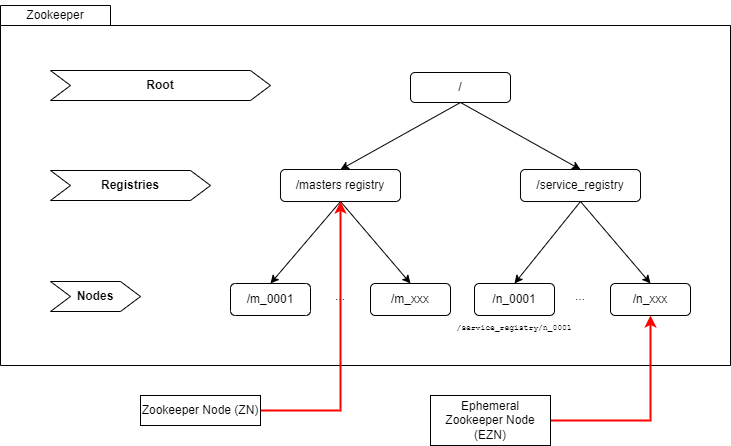
\includegraphics[width=0.7\linewidth]{Backend/Zookeeper ZNodes.png}
            \caption{Zookeeper ZNodes structure}
            \label{fig:zookeeper_znodes}
        \end{figure}
        
        \textbf{Watchers}
        
        A observer can be given to any ZN. This watcher observes for any change in the given ZN as shown in figure \ref{fig:zookeeper_watchers}, for instance nodes creation, deletion, data change and finally, addition or removal of child ZNodes. The watch API will notify the listener and this could be handled according to the requirements. The main drawback of ZK's watch implementation is that once triggered, the client must place a new one to continue using the feature.
        
        \begin{figure}[H]
            \centering
            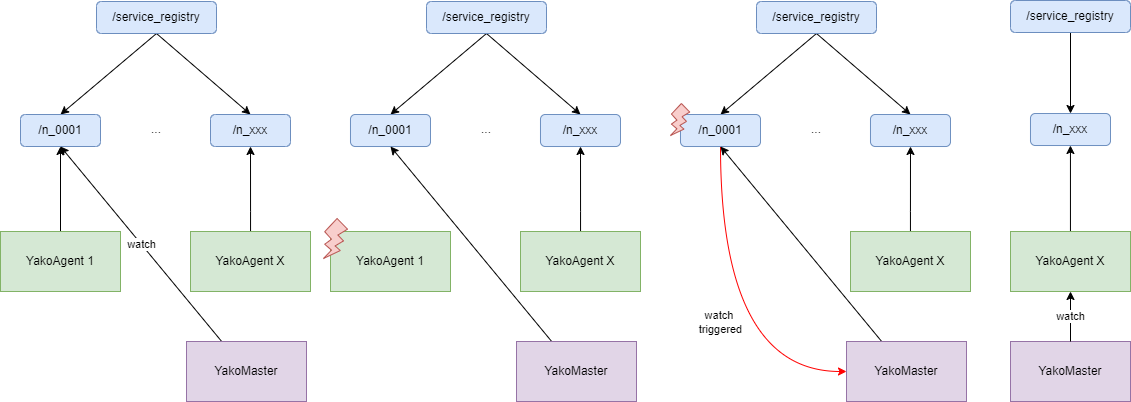
\includegraphics[width=\linewidth]{/Backend/Zookeeper Watchers.png}
            \caption{Zookeeper Watchers}
            \label{fig:zookeeper_watchers}
        \end{figure}
    
    \subsubsection{YakoMaster} \label{yakomaster}
        A YakoMaster can considered as the brain of the entire system because it coordinates all the computational resources. There must be at least on of its kind. The following list highlights this server's most important tasks:
        
        \begin{itemize}
            \item Serves and exposes an API for the client to interact with the system
            \item Keeps track of the current state of the platform at every single moment
            \item Identifies the best node to deploy the application according to the requirements
            \item Handles application upload and deployment
        \end{itemize}
        
        It supports two types of computing apparatus, conventional YakoAgent [\ref{yakoagent}] and YakoAgent (IoT) [\ref{yakoagentiot}] for Internet of Things devices. To enable support for both categories of devices, two standards have been used, gRPC communication for common devices and MQTT communication for IoT based ones.
        
        \subsubsubsection{System sequence diagram explanation}
            As shown in figure \ref{fig:yakomaster_sd}, on service start up, the agent tries to connect to ZK. If the connection has been successfully established, a singleton client is created for further interactions with the service registry.
            
            Attempts to create a master registry ZN, this node will be created once and only on the first YakoMaster instance startup because it is not an ephemeral but a persistent one. It then register itself to the masters registry and a Zookeeper Node Universally Unique Identifier (znUUID) is provided back. This registers' sole purpose is to track all the coordinators in the cluster and for security purposes.
            
            After that, a registration of UNIX signals processing handlers are established, this captures and processes SIGINT, SIGKILL, SIGTERM events. On YakoMaster Interrupt / Kill / Terminate, the program will gracefully shutdown all the connections to the ZK Service Registry by de-registering itself from it with the znUUID, shutdown the connection with the Mosquitto MQTT broker, gracefully shutdown the gRPC client to all the gRPC servers, shutdown the API server and finally close its running process.
            
            The next procedures are to register to the Mosquitto MQTT broker, serves the API and finally, it stops at an event loop awaiting for new services event. 
            
            \begin{figure}[H]
                \centering
                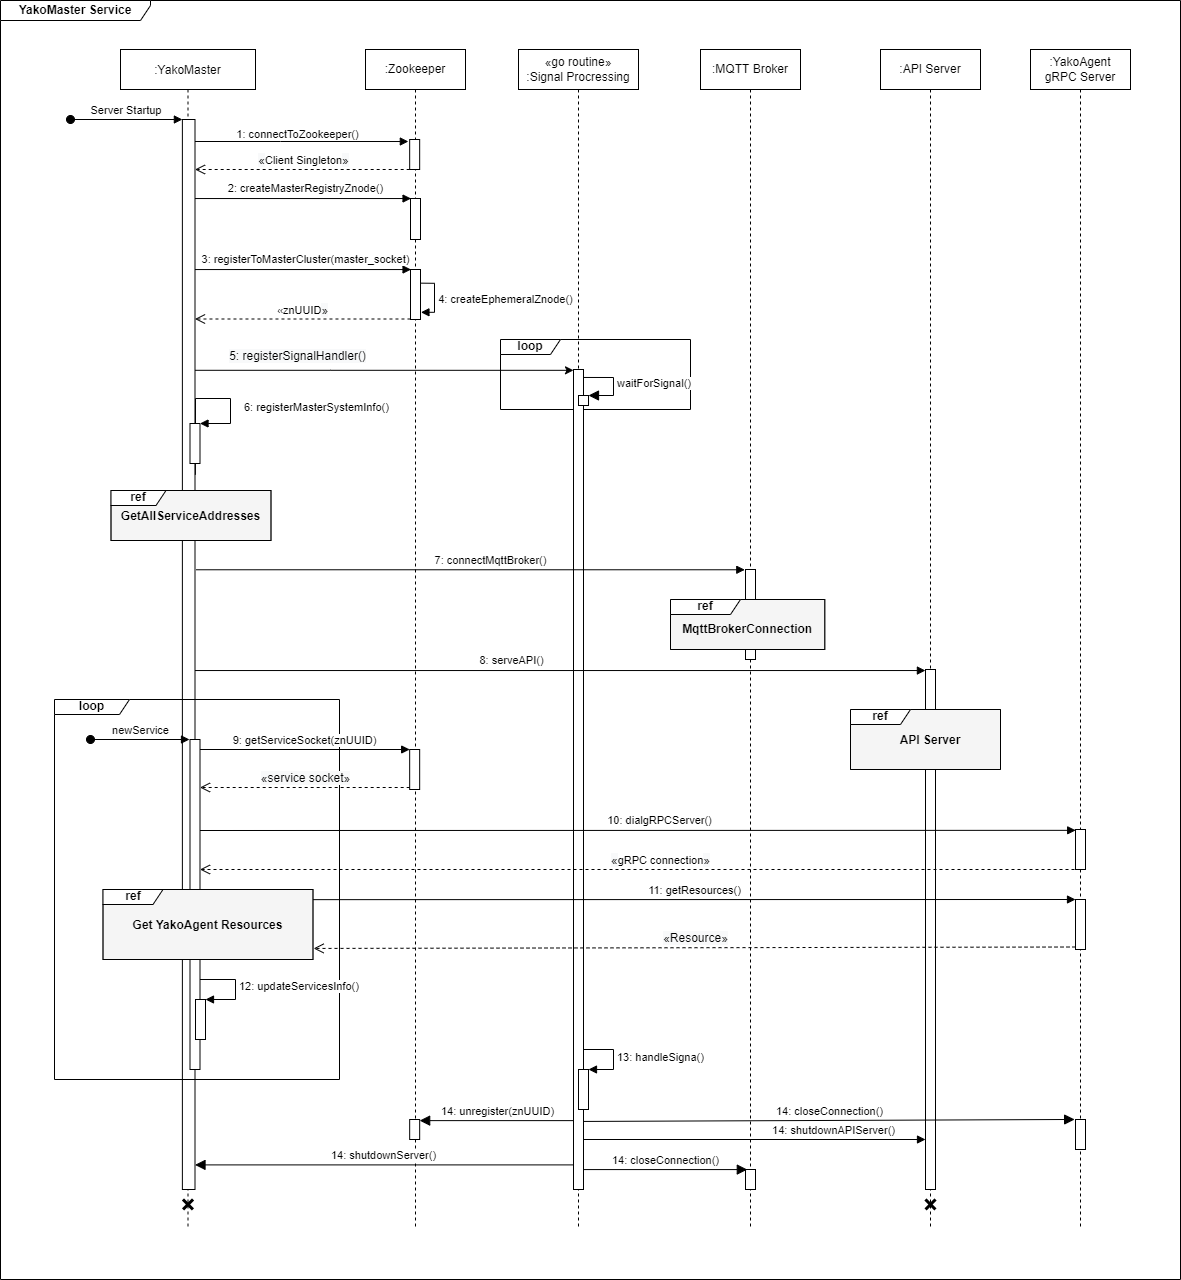
\includegraphics[width=0.8\linewidth]{Images/Backend/YakoMaster SD.png}
                \caption{YakoMaster service sequence diagram}
                \label{fig:yakomaster_sd}
            \end{figure}
            
            Between the signal handler registration and the Mosquitto client connection, YakoMaster will create a new Go routine which will get all services addresses as shown in Figure \ref{fig:services_addresses_sd}. In this thread, the program will get all children from the service registry and ZK will add a watch to the service registry ZN (/service\_registry), figure \ref{fig:zookeeper_znodes}. For each obtained children (service in our cluster), the orchestrator will proceed to get its socket, the meta-data information stored in ZK. If the child did not exist previously, it will prepare and allocate memory to store that YakoAgent's information. It then adds an observer to the child for ZK events.
            Internally, YakoMaster uses a map data structure to efficiently store the available computing YakoAgents and its system information is retrieved back in \(O(1)\) time using the znUUID as the key.
        
            \begin{figure}[H]
                \centering
                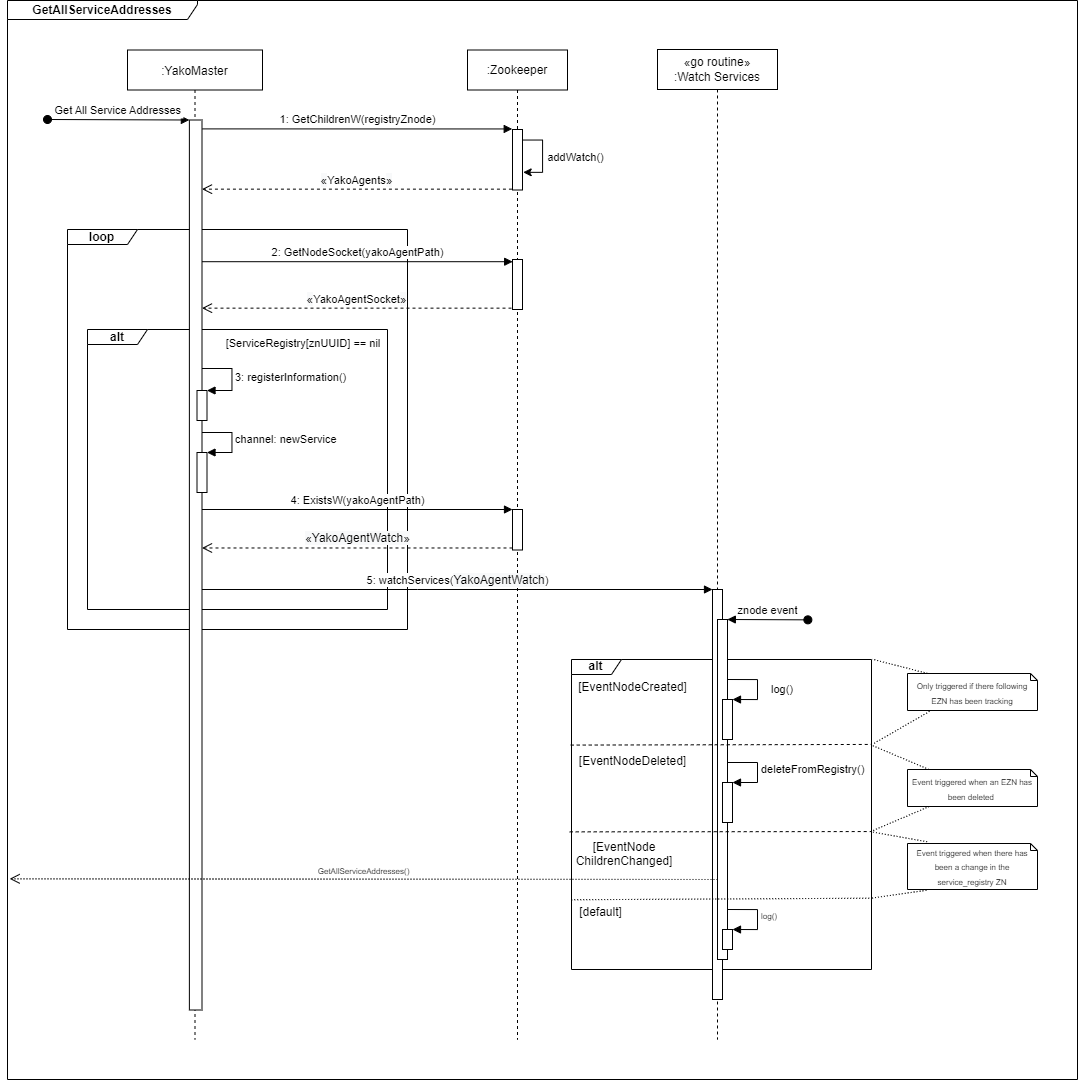
\includegraphics[width=\linewidth]{Images/Backend/GetAllServicesAddresses SD.png}
                \caption{Get all services addresses sequence diagram}
                \label{fig:services_addresses_sd}
            \end{figure}
            
            The possible ZK events are handled by another Go routine and the event types are listed below:
            
            \begin{itemize}
                \item \textbf{EventNodeCreated} will be triggered on YakoAgent registration only if the following EZN was being tracked.
                \item \textbf{EventNodeChildrenChanged} will be triggered on new YakoAgent registration. It will perform the flow from figure \ref{fig:services_addresses_sd}, again.
                \item \textbf{EventNodeDeleted} will be triggered on YakoAgent de-registration and disconnection. The handler will de-allocate the memory used in the map.
            \end{itemize}
        
            If the system detects a new YakoAgent, this will unblock the event loop from the main program and will connect to the gRPC server. On connection established it will send a request asking that specific agent to provide its resources information, as illustrated in figure \ref{fig:get_yakoagent_resources_sd}. Lastly, the newly obtained information will be updated, also in constant \(O(1)\) time, in the internal map.
        
            \begin{figure}[H]
                \centering
                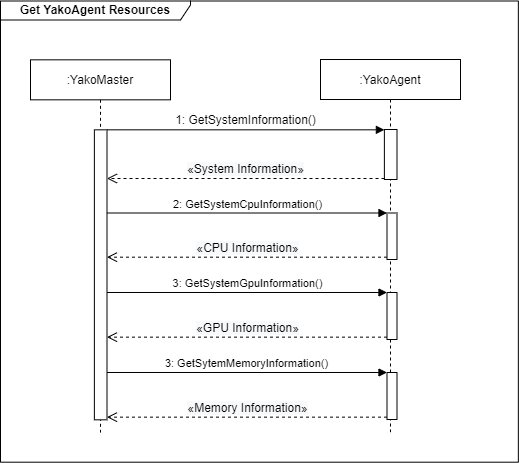
\includegraphics[width=0.5\linewidth]{Images/Backend/Get YakoAgent Resources SD.png}
                \caption{Get YakoAgent resources sequence diagram}
                \label{fig:get_yakoagent_resources_sd}
            \end{figure}
        
        \subsubsubsection{API Server}
            A REST API \cite{redhat_que_2020}, which is the gateway to interact with orchestrator of the cluster, is served with Gin Gonic Golang framework \cite{gin_gonic_gin_nodate}. The documentation is exposed at <yakomaster\_ip>:<yakomaster\_port>/docs and can be accessed with any browser or API testers like curl \cite{curl_curl_nodate} or Postman \cite{postman_postman_nodate} / Hoppscotch \cite{hoppscotch_hoppscotchhoppscotch_2022}. The format complies with the swagger and OpenAPI standard \cite{openapi_initiative_openapi_nodate}.
            
            \begin{figure}[H]
                \centering
                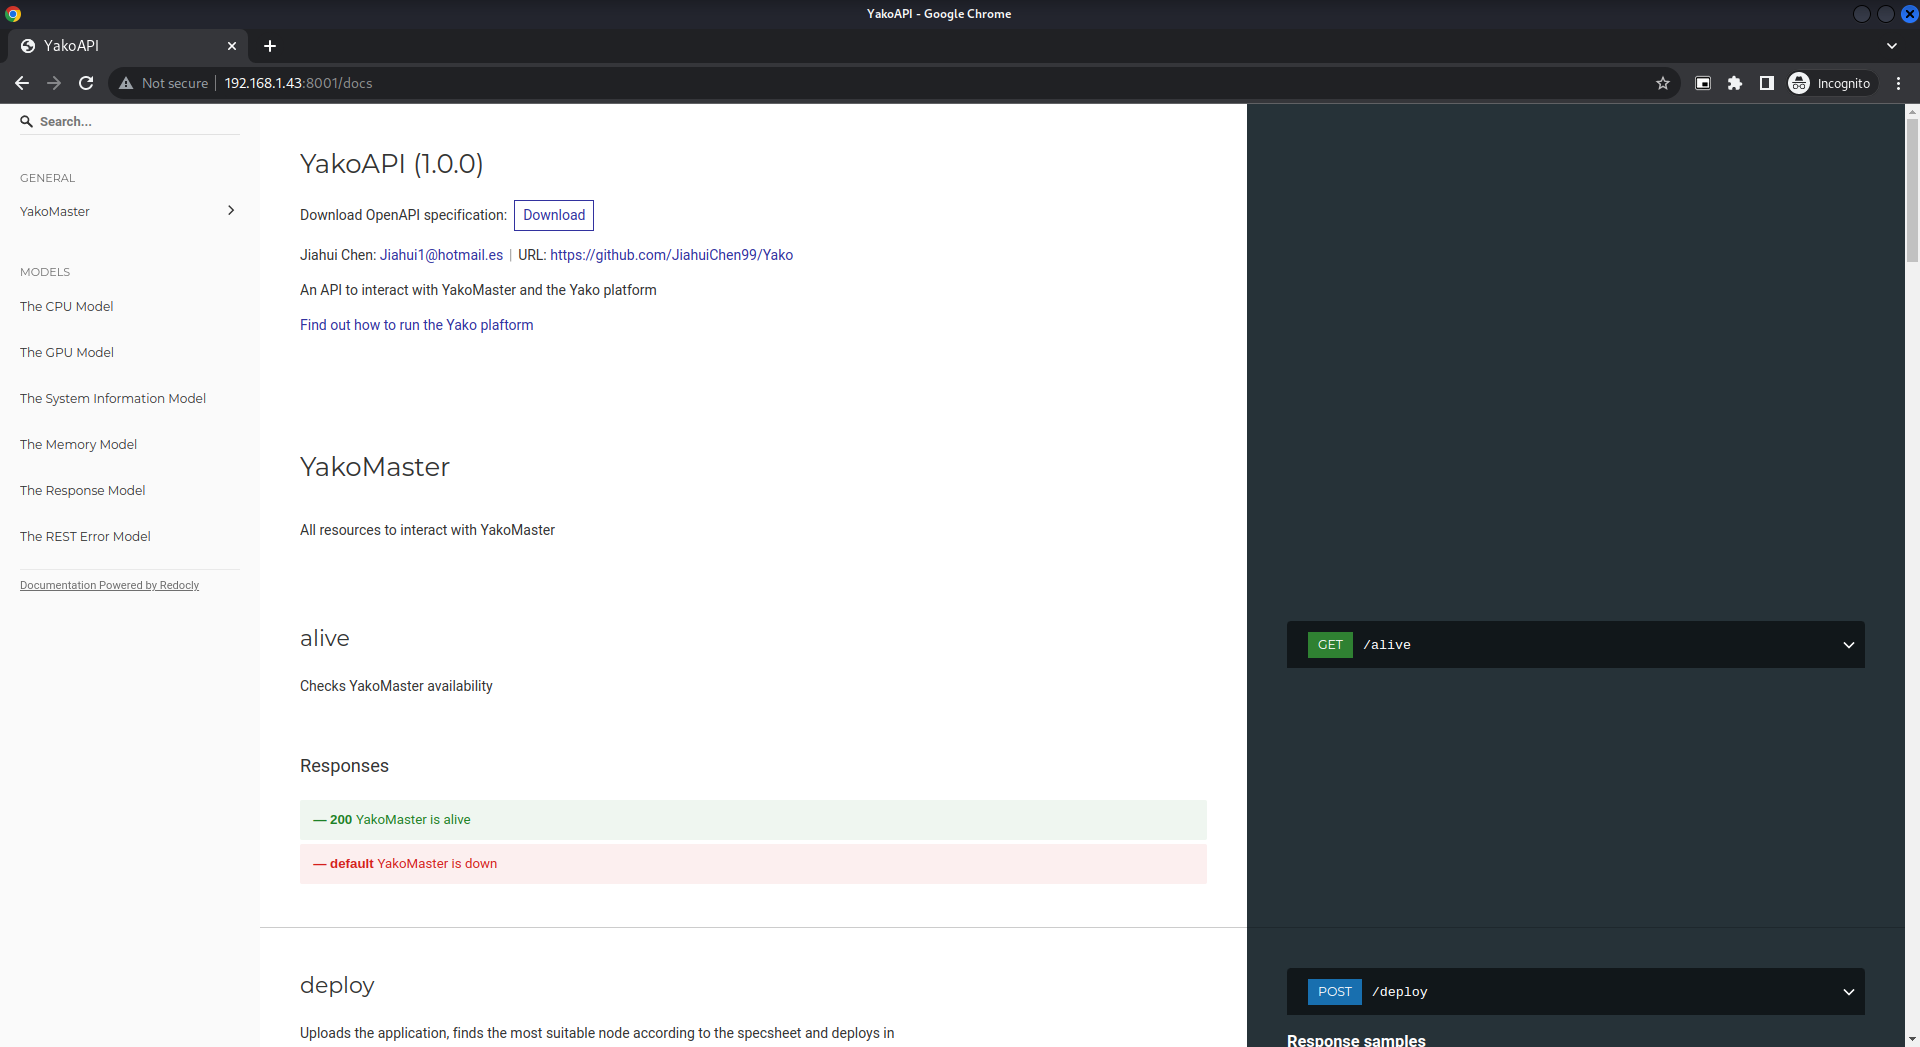
\includegraphics[width=\linewidth]{Images/Backend/YakoAPI.png}
                \caption{YakoAPI}
                \label{fig:yako_api}
            \end{figure}
            
            As depicted in the following figure \ref{fig:postman}, Postman software has been used to conduct API testing during the project development.
            
            \begin{figure}[H]
                \centering
                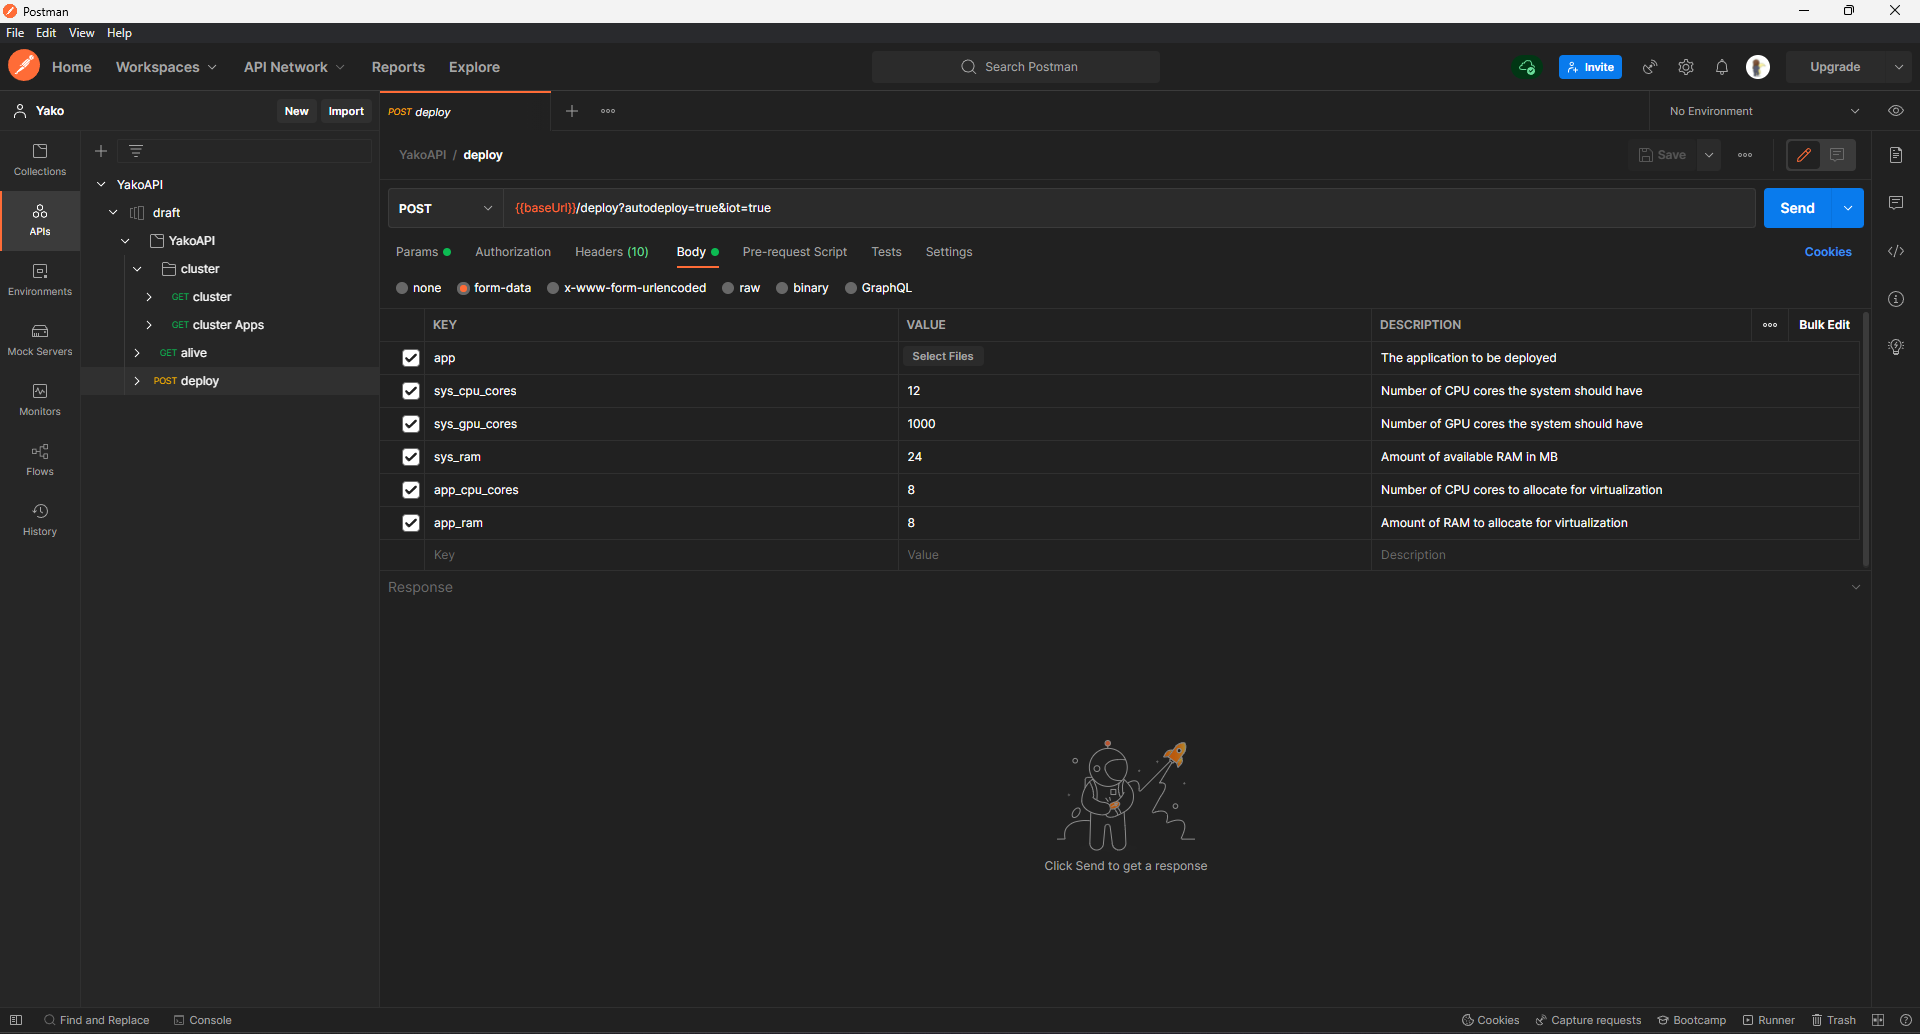
\includegraphics[width=\linewidth]{Images/Backend/Postman.png}
                \caption{Postman API testing}
                \label{fig:postman}
            \end{figure}
            
            
            Code snippet \ref{code:api_server} and figure \ref{fig:api_server_sd} sequence diagram show the API server starting process from the main YakoMaster procedure in figure \ref{fig:yakomaster_sd}.

            \begin{figure}[H]
                \begin{minipage}{0.5\textwidth}
                    \inputminted[
                        frame=lines,
                        framesep=2mm,
                        baselinestretch=1,
                        bgcolor=LightGray,
                        fontsize=\footnotesize,
                        breaklines=true,
                        linenos
                    ]{go}{Code/APIServer.go}
                    \subcaption{API Server}
                    \label{code:api_server}
                \end{minipage}
                \begin{minipage}{0.5\textwidth}
                    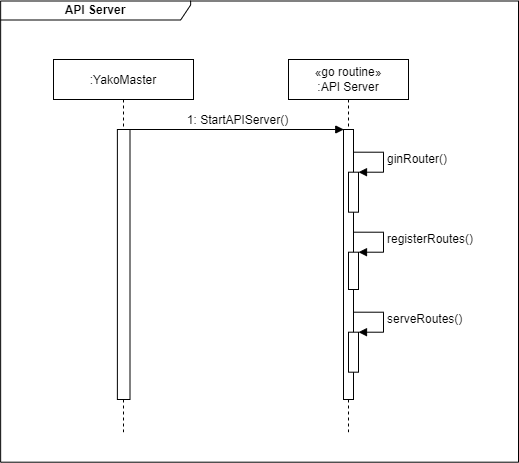
\includegraphics[width=\textwidth]{Images/Backend/API Server SD.png}
                    \subcaption{API Server sequence diagram}
                    \label{fig:api_server_sd}
                \end{minipage}
                \label{fig:api_server}
                \caption{API server}
            \end{figure}
            
            
            \subsubsubsubsection{Routes controller}
                The exposed routes of the API are defined in routing.go file and the following table \ref{tab:api_endpoints} compiles all the available endpoints and summarizes information related to these routes. Each of the endpoints have an associated controller which will perform business logic.
                
                \begin{table}[H]
                    \centering
                    \caption{YakoAPI Endpoint}
                    \begin{tabular}{|l|l|l|l|}
                    \hline
                    \rowcolor[HTML]{C0C0C0} 
                    \textbf{Route endpoint} & \textbf{Method} & \textbf{Controller} & \textbf{Brief Comment} \\ \hline
                    /alive & GET & IsAlive & Pings the server and checks for its status \\ \hline
                    /deploy & POST & UploadApp & Uploads the application and deploys the it \\ \hline
                    /cluster & GET & Cluster & Retrieve all the cluster information \\ \hline
                    /cluster/apps & GET & GetClusterApps & Retrieve all deployed applications \\ \hline
                    \end{tabular}
                    \label{tab:api_endpoints}
                \end{table}
            
                \textbf{IsAlive}
                
                IsAlive is a simple route to check whether the orchestrator is operating or down, it is used before uploading an application in front-end software. The return value of this will be a HTTP Status OK code: 200 for a, or will timeout HTTP Timeout Code 408 otherwise.
                
                \begin{code}
                    \inputminted[
                        frame=lines,
                        framesep=2mm,
                        baselinestretch=1,
                        bgcolor=LightGray,
                        fontsize=\footnotesize,
                        breaklines=true,
                        linenos
                    ]{go}{Code/API/alive.go}
                    \caption{IsAlive handler - alive.go}
                    \label{code:alive}
                \end{code}
            
                \textbf{UploadApp}
                
                As the controller's name suggest, this endpoint is to be requested when the system administrator wants to upload and deploy an application to the system.
                
                \begin{code}
                    \inputminted[
                        frame=lines,
                        framesep=2mm,
                        baselinestretch=1,
                        bgcolor=LightGray,
                        fontsize=\footnotesize,
                        breaklines=true,
                        linenos
                    ]{go}{Code/API/uploadapp.go}
                    \caption{UploadApp handler - deploy.go}
                    \label{code:uploadapp}
                \end{code}
            
                The request's header sent to the UploadApp endpoint must contain a Content-Type \cite{mdn_content-type_nodate} property of type "multipart/form-data", this will tell the server the data type of the request. The application to be deployed must be attached to the form in the app field. The client accepts application/json content type back.
                
                \begin{table}[H]
                    \centering
                    \caption{UploadApp HTTP request headers}
                    \begin{tabular}{|l|l|l|}
                    \hline
                    \rowcolor[HTML]{C0C0C0} 
                    \textbf{Key} & \textbf{Value} & \textbf{Description} \\ \hline
                    Content-type & multipart/form-data & The content of the request i \\ \hline
                    Accept & application/json & The endpoint accepts JSON formatting \\ \hline
                    \end{tabular}
                    \label{tab:uploadapp_headers}
                \end{table}
        
                Currently, the supported request parameters are Auto-deploy and IoT. These are compulsory and must be set into the request. As described in the table \ref{tab:uploadapp_params}, autodeploy is a variable of boolean type and setting iot to true will only select YakoAgents (IoT), filtering out non IoT devices. Platform and architecture properties are yet to be supported, and will apply OS and CPU architecture (x86-64, ARM, etc \cite{academic_list_nodate}) filtering, respectively.
                
                \begin{table}[H]
                    \centering
                    \caption{UploadApp HTTP request parameters}
                    \begin{tabular}{|l|l|l|l|}
                    \hline
                    \rowcolor[HTML]{C0C0C0} 
                    \textbf{Key} & \textbf{Support} & \textbf{Type} & \textbf{Description} \\ \hline
                    autodeploy & Supported & Boolean & Automates the application deployment \\ \hline
                    iot  & Supported & Boolean & Applies IoT devices filtering \\ \hline
                    platform & Unsupported & String & Applies OS filtering  \\ \hline
                    architecture & Unsupported & String & Applies CPU architecture filtering  \\ \hline
                    \end{tabular}
                    \label{tab:uploadapp_params}
                \end{table}
                
                Table \ref{tab:uploadapp_body} lists all the accepted form keys by the server. Setting these is compulsory for the server to conduct the matching. There are two types of keys: System (sys\_xxx) which refers to system requirements, this information will be used to find the most suitable node, and App (app\_xxx) used for virtualization which is not supported yet. Other keys could be added in the future to apply finer searching granularity, for instance, latency, disk capacity, disk I/O speeds, RAM speeds, to name a few.
            
                \begin{table}[H]
                    \centering
                    \caption{UploadApp HTTP request body}
                    \begin{tabular}{|l|l|l|}
                    \hline
                    \rowcolor[HTML]{C0C0C0} 
                    \textbf{Key} & \textbf{Type} & \textbf{Description} \\ \hline
                    app & File & The application to be deployed \\ \hline
                    sys\_cpu\_cores & Text & Number of CPU cores the system should have \\ \hline
                    sys\_gpu\_cores & Text & Number of GPU cores the system should have \\ \hline
                    sys\_ram & Text & Amount of available RAM in MB  \\ \hline
                    app\_cpu\_cores & Text & Number of CPU cores to allocate for virtualization \\ \hline
                    app\_ram & Text & Amount of RAM to allocate for virtualization \\ \hline
                    \end{tabular}
                    \label{tab:uploadapp_body}
                \end{table}
                
                An example of such request is shown in Code snippet \ref{code:uploadapp_request}, it is a POST petition that accepts form-data as its content type. The selected application is attached to the app key in the form. And the preferred node to run it, should have 12 CPU cores, 1000 GPU cores and 24 GB of RAM, and allocate a total of 8 CPU cores and 8192 MB of RAM for virtualization.
            
                \begin{code}
                    \inputminted[
                        frame=lines,
                        framesep=2mm,
                        baselinestretch=1,
                        bgcolor=LightGray,
                        fontsize=\footnotesize,
                        breaklines=true,
                        linenos
                    ]{bash}{Code/API/uploadapp.sh}
                    \caption{UploadApp POST request example with cURL}
                    \label{code:uploadapp_request}
                \end{code}
                
                On request handle, source code \ref{code:uploadapp}, YakoMaster will compile the system's and app's requirements from the provided form. Once the information is gathered, the orchestrator will find, by default, the top 3 most suitable nodes. If auto-deploy is enabled, YakoMaster will handle the deployment automatically, otherwise the application will remain uploaded in the system and could be deployed later on. The orchestrator will call the first node and send the application via gRPC streaming upload \ref{rpc_deploytoagent} if "iot" parameter is not set. Alternatively, if the deployment is to a YakoAgent (IoT), the file would be sent via custom socket streaming to the YakoAgent server as shown in Upload Application reference block from figure \ref{fig:yakoagentiot_sd}. Finally, the endpoint will render an array of recommended nodes back to the client, an example is shown in snippet \ref{code:uploadapp_response}.
                
                \begin{code}
                    \inputminted[
                        frame=lines,
                        framesep=2mm,
                        baselinestretch=1,
                        bgcolor=LightGray,
                        fontsize=\footnotesize,
                        breaklines=true,
                        linenos
                    ]{json}{Code/API/uploadapp_response.json}
                    \caption{UploadApp POST response example}
                    \label{code:uploadapp_response}
                \end{code}
            
            % Find best nodes algorithm
            The heuristic applied to find the best nodes is simple and straightforward. YakoMaster will examine all the available nodes in the platform, firstly by filtering out those that do not match the filtering "iot" parameter. For each of the remaining nodes, the orchestrator will assert if it complies with the properties that the system administrator has set in the form. Currently the system only checks the CPU cores and available RAM. The more it complies the more brownie points will be given to the node. These brownie points will be the determinant factor for the priority queue as a max-heap. In other words, the first node in the heap will be the one with the most brownie points, the YakoAgent that satisfies the most with the requirements. At the current state of the project, with only 2 parameters to check, it is possible that many agents would result in a tie. To solve such event, more parameters are planned to be implemented, as shown previously in table \ref{tab:uploadapp_params}. As more properties to check the less likelihood will that happen. To further decrease that unwanted event, a weighting system and/or strict parameters (parameters that must be complied) could be applied to break the deadlock.
            
            \begin{code}
                \inputminted[
                    frame=lines,
                    framesep=2mm,
                    baselinestretch=1,
                    bgcolor=LightGray,
                    fontsize=\footnotesize,
                    breaklines=true,
                    linenos
                ]{go}{Code/API/findyakoagents.go}
                \caption{Find Top YakoAgents - deploy.go}
                \label{code:uploadapp}
            \end{code}
            
            \textbf{Cluster}
            
            This endpoint will dump all the information recorded in YakoMaster's internal services map. The structure includes all the YakoMasters and YakoAgents. The information will be up to date with at most 10 seconds of age.
            
            \begin{code}
                \inputminted[
                    frame=lines,
                    framesep=2mm,
                    baselinestretch=1,
                    bgcolor=LightGray,
                    fontsize=\footnotesize,
                    breaklines=true,
                    linenos
                ]{go}{Code/API/cluster.go}
                \caption{Cluster handler - cluster.go}
                \label{code:alive}
            \end{code}
            
            An example of cluster GET request response is shown below, in snippet \ref{code:cluster_response}.
            
            \begin{code}
                \inputminted[
                    frame=lines,
                    framesep=2mm,
                    baselinestretch=1,
                    bgcolor=LightGray,
                    fontsize=\footnotesize,
                    breaklines=true,
                    linenos
                ]{json}{Code/API/cluster_response.json}
                \caption{Cluster GET response example}
                \label{code:cluster_response}
            \end{code}
            
            \textbf{GetClusterApps}
            
            This endpoint will read YakoMaster's working directory, where all the previously uploaded applications have been stored, and render back the list. This information is used in the Dashboard \ref{fig:dashboard_ui} view, and could allow system administrators to perform an application re-deployment without having to re-upload it.
            
            \begin{code}
                \inputminted[
                    frame=lines,
                    framesep=2mm,
                    baselinestretch=1,
                    bgcolor=LightGray,
                    fontsize=\footnotesize,
                    breaklines=true,
                    linenos
                ]{go}{Code/API/get_cluster_apps.go}
                \caption{GetClusterApps handler - cluster.go}
                \label{code:alive}
            \end{code}
            
            An example of the requested applications list is shown in response snippet \ref{code:clusterapps_response}.
            
            \begin{code}
                \inputminted[
                    frame=lines,
                    framesep=2mm,
                    baselinestretch=1,
                    bgcolor=LightGray,
                    fontsize=\footnotesize,
                    breaklines=true,
                    linenos
                ]{json}{Code/API/getclusterapps_response.json}
                \caption{Cluster Apps GET response example}
                \label{code:clusterapps_response}
            \end{code}
    
        \subsubsubsection{MQTT broker connection}
            Figure \ref{fig:mqtt_broker_connection_sd} depicts the process of YakoMaster's connection to the MQTT broker. 
            Eclipse Mosquitto \cite{eclipse_eclipse_2018} has been used for this purpose and uses the publish/subscribe pattern. The main benefit of this method, is that the orchestrator does not need to repeatedly poll the publishers (YakoAgent IoT) for updates.
            The IP and port of the broker is provided as programs arguments on startup. A new MQTT client configuration is created with the builder software pattern. With the generated configuration, a connection is then established with the broker. Once connected YakoMaster subscribes to all the available topics. All the available topics a YakoAgent publishes are listed in section \ref{yakoagent}. 
        
            \begin{figure}[H]
                \centering
                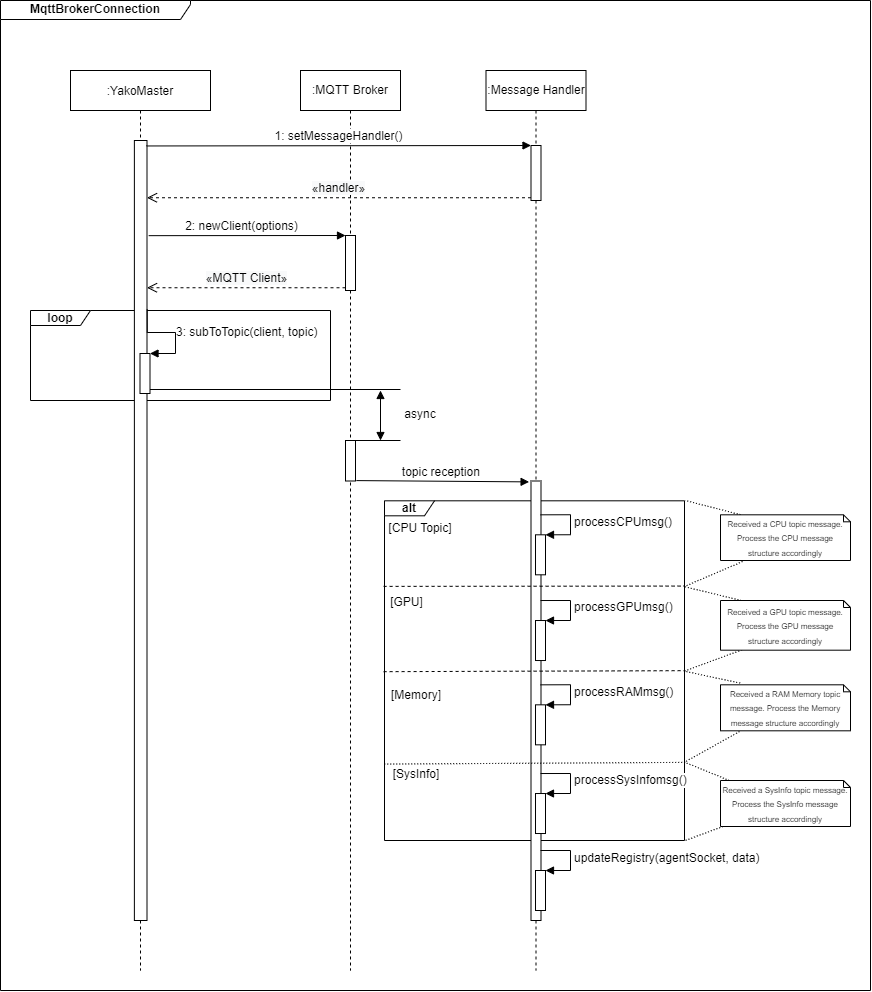
\includegraphics[width=0.95\linewidth]{Images/Backend/MQTT Connection SD.png}
                \caption{Connect to MQTT Broker sequence diagram}
                \label{fig:mqtt_broker_connection_sd}
            \end{figure}
            
            The receiving of the topics are asynchronous and can happen at any time during the runtime. Once a topic is received, a message handler \ref{code:mqtt_message_handler} processes it. The messages have the following format:
            
            \[     \boxed{/topic/+/resource}    \]\\
            
            The first topic level indicates that it is a topic, succeeded by a single-level wildcard, the \textbf{+} sign, and finally the second topic level indicates the resource that its being received. The wild-card acts as a variable and is substituted by the socket of the publisher.
            With this information the message handler from YakoMaster can determine the origin of the message and the resource type information that the packet contains.
            The MQTT published messages payload is serialized in JSON format, but later releases support for protocol buffers could be supported to diminish network usage footprint.
        
            % processing code
            \begin{code}
                \inputminted[
                    frame=lines,
                    framesep=2mm,
                    baselinestretch=1,
                    bgcolor=LightGray,
                    fontsize=\footnotesize,
                    breaklines=true,
                    linenos
                ]{go}{Code/mqtt_message_handler.go}
                \caption{MQTT message handler}
                \label{code:mqtt_message_handler}
            \end{code}
    
    \subsubsection{YakoAgent} \label{yakoagent}
        A YakoAgent is a computational node, it is intended to be a node where applications will be deployed. Internally the YakoAgent starts a gRPC server which implements a service called \textbf{NodeService}. The NodeService describes a series of Remote Procedures calls which must be implemented depending on the need. The implementation of these RPC will be system dependant, how the resources are described differs from one Operating System to another. For instance, to get system CPU data, in Linux distributions this information is located in the /proc/cpuinfo file, while in Microsoft Windows OSes, to read that information, a query to Performance Counters \cite{karl-bridge-microsoft_performance_nodate} or Process Status API \cite{karl-bridge-microsoft_process_nodate} must be made instead.
        
        \begin{figure}[H]
            \centering
            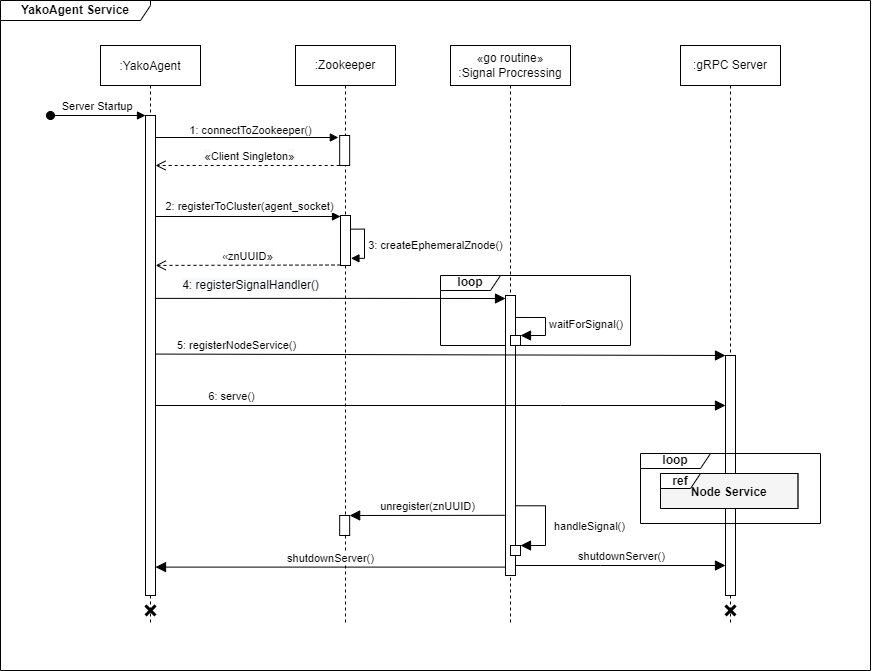
\includegraphics[width=0.8\linewidth]{Backend/YakoAgent SD.png}
            \caption{YakoAgent service sequence diagram}
            \label{fig:yakoagent_sd}
        \end{figure}
        
        Both, service and RPCs are defined in a \textit{.proto} file shared across all the systems that uses gRPC in the Yako platform, YakoMaster and YakoAgent. 
        Most of the information system resources information are retrieved from the /proc folder, which is a special folder, a Virtual File System (VFS) instead of a physical File System (FS) mounted on boot time.
        
        \begin{code}
            \inputminted[
                frame=lines,
                framesep=2mm,
                baselinestretch=1,
                bgcolor=LightGray,
                fontsize=\footnotesize,
                linenos
            ]{c}{Code/node.proto}
            \caption{YakoAgent services and RPCs API}
            \label{code:rpc_services}
        \end{code}
        
        The use gRPC as the communication protocol for the agents is due to its widely adoption in the cloud, distributed, computing context. gRPC can efficiently connect services across distributed environments. Its ubiquitous adoption, support for multi-platforms and high performance makes it the best candidate.
        
        \textbf{GetSystemInformation RPC}
        
        This RPC will gather generic information of the system where the YakoAgent is running on. Internally it makes a \textit{uname} system call \cite{mackenzie_uname1_nodate}.
        The OS presumably knows its name, release, version and hardware. Part of this information can be read from /proc/sys/kernel/\{ostype, hostname, osrelease, version, domainname\}.
        
        
        \begin{code}
            \inputminted[
                frame=lines,
                framesep=2mm,
                baselinestretch=1,
                bgcolor=LightGray,
                fontsize=\footnotesize,
                linenos
            ]{go}{Code/sysinfo.go}
            \caption{System Information model - sysinfo.go}
            \label{code:sysinfo_model}
        \end{code}
        
        
        \textbf{GetSystemCpuInformation RPC}
        
        This RPC will gather CPU related information. The information is located in the /proc/cpuinfo path. As shown in the Source Code \ref{code:cpu_model}, the most relevant information (name, cores number, socket, list of cores) of the CPU is retained.
        
        \begin{code}
            \inputminted[
                frame=lines,
                framesep=2mm,
                baselinestretch=1,
                bgcolor=LightGray,
                fontsize=\footnotesize,
                breaklines=true,
                linenos
            ]{go}{Code/cpu.go}
            \caption{CPU model - cpu.go}
            \label{code:cpu_model}
        \end{code}
        
        \textbf{GetSystemGpuInformation RPC}
        
        This RPC will retrieve GPU related information if any. Not all systems have GPU support, that is the reason why the program first checks for a GPU availability if none a log will be prompted to the terminal. The platform currently supports NVIDIA graphical processing units, and the correct drivers must be installed in order to perform the lookup. If all the previous conditions are met, the folder will be checked. The structure contains the following properties.
        
        \begin{code}
            \inputminted[
                frame=lines,
                framesep=2mm,
                baselinestretch=1,
                bgcolor=LightGray,
                fontsize=\footnotesize,
                breaklines=true,
                linenos
            ]{go}{Code/gpu.go}
            \caption{GPU model - gpu.go}
            \label{code:gpu_model}
        \end{code}
        
        \textbf{GetSystemMemoryInformation RPC}
        
        This RPC will report the amount of Random Access Memory (RAM) the system has installed. Information about the consumed and availability of both RAM and Swap virtual memory, as described in Source Code \ref{code:memory_model}.
        
        \begin{code}
            \inputminted[
                frame=lines,
                framesep=2mm,
                baselinestretch=1,
                bgcolor=LightGray,
                fontsize=\footnotesize,
                breaklines=true,
                linenos
            ]{go}{Code/memory.go}
            \caption{Memory model - memory.go}
            \label{code:memory_model}
        \end{code}
        
        % DeployApp gRPC
        \textbf{DeployAppToAgent RPC} \label{rpc_deploytoagent}
        
        The YakoAgent service follows a life-cycle depicted in Figure \ref{fig:yakoagent_sd} during its lifespan.
        On server start up, before operating, it first connects to Apache Zookeeper to obtain a singleton client, which will be used during the entire session to communicate with the Service Registry utility from Zookeeper.
        Shortly after the client obtaining, it registers to the Service Registry, this will dispatch an event that will create a sequential Ephemeral Zookeeper Node (EZN). After its completion a unique identifier (znUUID) will be returned back to the agent. This key has various purposes, for instance, node identification, node de-registration, node watcher. The value  of each newly generated identifier will be unique and auto-incremented, following n\_<auto\_increment\_ID> pattern.
        ZK has support for EZNs, these are special ZNodes that only exists as long as the session that created them is active. If the YakoAgent is disconnected either due to a failure or manual shut-down, the session ends, consequently the ZN is deleted. This is reported back and notified to the YakoMaster which is constantly monitoring the state of the entire system.
        After that step, the service will register a signal handler to process all incoming signals either from the system administrator (User) or from the OS (External Event), at any time.
        The Node Service is then registered to the gRPC Server following by a service exposure.
        To stop YakoAgent from operating, three signals can be used, these are Signal Interrupt (SIGINT), Signal Terminate (SIGTERM) and Signal Kill (SIGKILL).
        
        \begin{figure}[H]
            \centering
            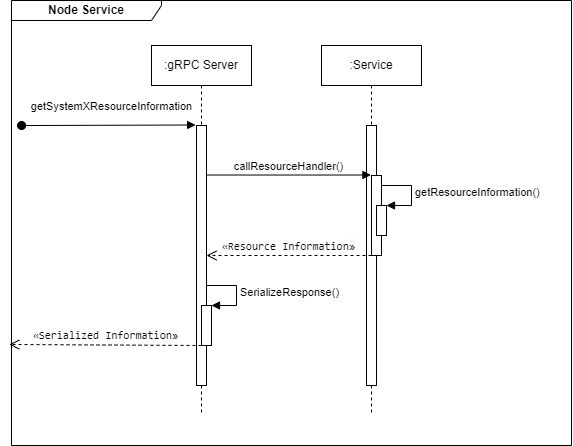
\includegraphics[width=0.8\linewidth]{Backend/NodeService SD.png}
            \caption{YakoAgent gRPC service sequence diagram}
            \label{fig:yakoagent_sd}
        \end{figure}

    \subsubsection{YakoAgent (IoT)} \label{yakoagentiot}
        YakoAgent (IoT) is a variant of the previous server, specifically designed to support IoT devices. It replaces the gRPC for MQTT \cite{oasis_mqtt_nodate} message queues, which implements the publish/subscribe pattern \cite{camp_guide_nodate}.
        As opposed to the standard YakoAgent, this server does not need to connect to the Service Registry to make its appearance in the system. It connects to the MQTT broker and periodically publishes its own system resources, the default timed reporting is 10 seconds but a higher or lower value could be set according to the system preferences.
        
        The following list enumerates the different topics available for YakoAgents (IoT) to self report its resources to the YakoMaster.
        
        \begin{itemize}
            \item \textbf{topic/<agent\_socket>/cpu:} To report system's CPU related information
            \item \textbf{topic/<agent\_socket>/gpu:} To report system's GPU (if any) information
            \item \textbf{topic/<agent\_socket>/memory:} To report system's RAM memory
            \item \textbf{topic/<agent\_socket>/sysinfo:} To report system generic information 
        \end{itemize}
        
        YakoMaster will be notified once there are information of any of the previous topics. It first performs a check and determines if the node exists in the service registry. If it was aware of it then it updates, otherwise it creates a new registry.
        
        \begin{figure}[H]
            \centering
            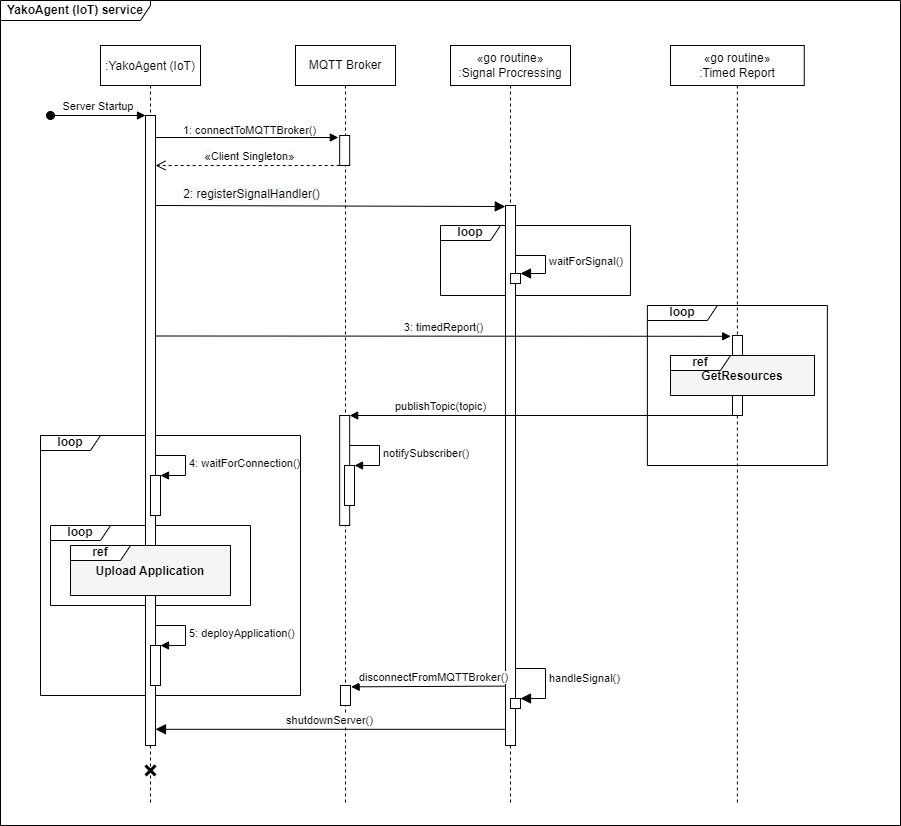
\includegraphics[width=0.8\linewidth]{Backend/YakoAgent IoT SD.png}
            \caption{YakoAgent IoT service sequence diagram}
            \label{fig:yakoagentiot_sd}
        \end{figure}
    
    \subsubsection{A more complex system}
        One of the core objectives for this platform to achieve, was to be a language agnostic, to work across platforms embracing the heterogeneity nature of the devices, hardware and software wise.
        
        A more complex system is presented in the following figure \ref{fig:complex_architecture}. Both YakoAgent and YakoAgent (IoT) clients could be developed with different languages according to the specific needs of the device. 
        
        It is known that the majority of IoT devices that constitute the edge layer of a distributed system are more resource constrained \cite{rajaee_iot_2017}. That is why system languages like Rust, C++ and Go with less memory consumption are more suitable, YakoAgent (IoT) clients for these language could be developed. For these devices to publish topics to the MQTT broker, a MQTT library of that language must be used, which all the aforementioned languages do have. 
        
        On the other hand, for YakoAgent nodes it is as simple as getting the different protocol buffers files and compiling for the programming language being used. Yako platform will support this software layer heterogeneity thanks to its unified messages protocols, gRPC with protocol buffers encoding and MQTT with JSON-encoding.
        
        \begin{figure}[H]
            \centering
            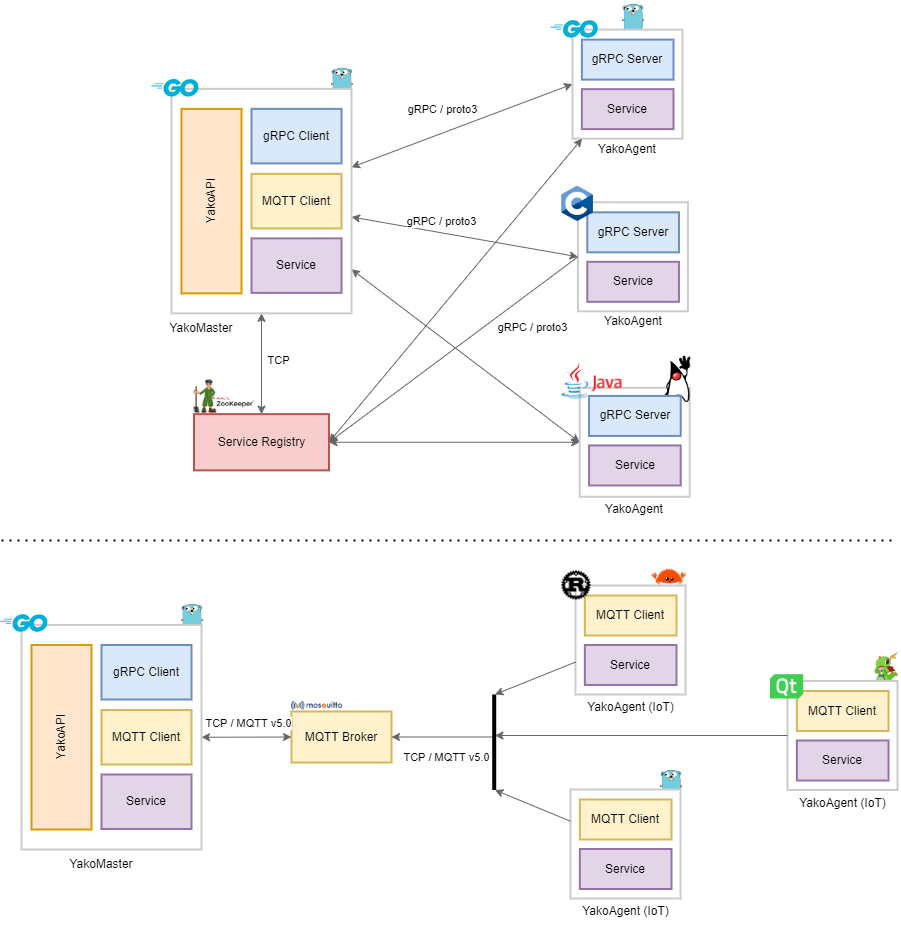
\includegraphics[width=0.95\linewidth]{Backend/Complex Architecture.png}
            \caption{Yako platform complex architecture (more heterogeneous): (top) other YakoAgent   (down): other YakoAgent (IoT) }
            \label{fig:complex_architecture}
        \end{figure}

    \subsection{Front-end}
    The front-end application is the control panel of the entire Yako platform. One of the key considerations when designing the application was, for this to be available to be used from any device. The software has been developed with the latest web technologies. It is a multi-platform application, hence, the software can be ran in diverse OS and supports mainstream platforms Microsoft Windows, Linux, Apple macOS, among others. This chapter discusses the process, iterations and changes the project has undergone. From the idea conception through the design process to the technology stack being used.
    
    \subsubsection{Architecture and Technologies}
        As presented in figure \ref{fig:simple_architecture} of the current chapter, the application user interface is built with VueJS \cite{vuejs_what_nodate}, a progressive web framework with the leverage of ElectronJS \cite{openjs_foundation_electron_nodate} which makes it possible to share one code base, build and distribute for different platforms.
        
        ElectronJS embeds Chromium and NodeJS into its binary. While Chromium is an open-source browser project in charge of displaying the content built with VueJS library, NodeJS is the server runtime environment that adds extensive APIs to access the file system and other OS features like networking and I/O. These characteristics are later used in different parts of the application, for instance, when accessing the file system to upload an application or when interacting with the platform API.
        
        \subsubsubsection{Application Architecture}
            The architecture of the front-end application is component-based \cite{dhaduk_component-driven_2021}. As opposed to monoliths, it adopts a modular approach that decomposes front-end UI, taking advantage of benefits like flexibility, responsibilities decoupling, similar to micro-services at the back-end.
        
            \begin{figure}[H]
                \centering
                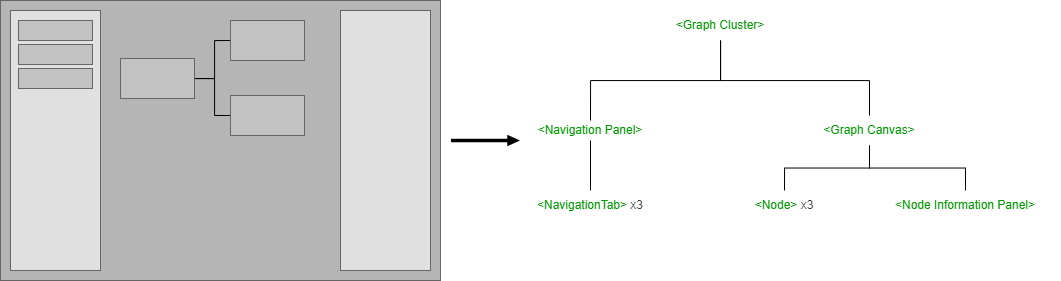
\includegraphics[width=\linewidth]{Frontend/components.png}
                \caption{Component-based UI}
                \label{fig:vue_components}
            \end{figure}
            
            Figure \ref{fig:vue_components} illustrates the Cluster Graph page, one of the views from the YakoUI application. Using VueJS components, enables splitting the UI into independent and reusable pieces. The application is then organized into a tree of nested components.
        
        \subsubsubsection{State handling}
            To handle the UI data changes, VueJS, listens to data change events and re-renders the UI to display that change. The communication between components is through the propagation of properties. which works fine for smaller scale applications. However, due to the natural growth of the software, Vuex \cite{vuejs_what_nodate}, a state management library has been used. The framework is the View component of the Flux pattern \cite{facebook_flux_nodate}.
            
            To modify the values of this global centralized store, an event must be triggered from the view, which would be sent to the dispatcher. The dispatcher then broadcasts the resulting payload which updates the store.
            
            \begin{figure}[H]
                \centering
                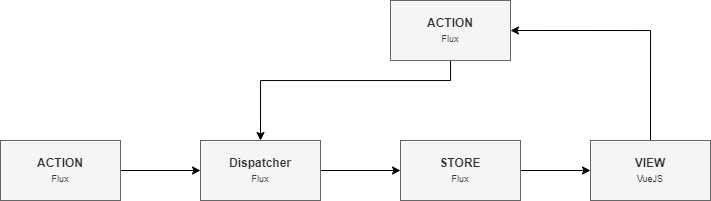
\includegraphics[width=\linewidth]{Frontend/flux.png}
                \caption{Vuex flux pattern}
                \label{fig:flux}
            \end{figure}
            
            At some parts of the project, the Provide / Inject \cite{vuejs_provide_nodate} feature has been used to pass data from the great-grandfather, namely any root component, to the leaf children components as shown in figure \ref{fig:provide_inject}, as opposed to components properties propagation which would lead to a prop-drilling issue.

            \begin{figure}[H]
                \begin{minipage}{0.5\textwidth}
                    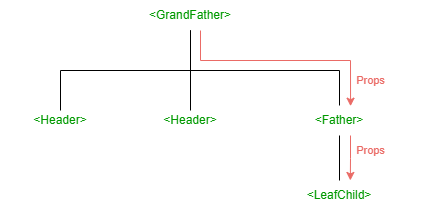
\includegraphics[width=\textwidth]{Images/Frontend/no_provide_inject.png}
                    \subcaption{Prop-drilling effect}
                    \label{code:no_provide_inject}
                \end{minipage}
                \begin{minipage}{0.5\textwidth}
                    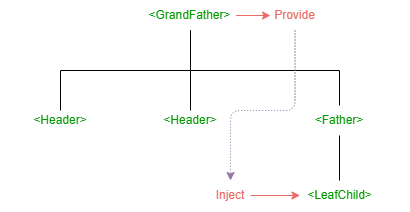
\includegraphics[width=\textwidth]{Images/Frontend/provide_inject.png}
                    \subcaption{Provide - Inject}
                    \label{fig:provide_inject}
                \end{minipage}
                \label{fig:props_propagation}
                \caption{Components properties propagation}
            \end{figure}
        
    
    \subsubsection{Project Structure}
        The project source code structure is divided into 5 big folders:
        
        \begin{itemize}
            \item \textbf{Pages:} Contains the views of the application. For the final software, Upload Application page, Dashboard page and page were developed
            \item \textbf{Components:} Contains all the source code for the developed components for the project
            \item \textbf{Router:} Contains the logic for switching the pages of the application
            \item \textbf{Services:} Contains API endpoints to interact with the Yako platform and other utilities logic used across the software
            \item \textbf{Store:} Logic of Vuex, the global state management
        \end{itemize}

        The following UML diagram shows the relationship of the different components used in the software.
        
        \begin{figure}[H]
            \centering
            \includegraphics[width=0.8\linewidth]{/Frontend/yakoui UML.png}
            \caption{YakoUI project UML}
            \label{fig:yakoui_uml}
        \end{figure}
        
        
    \subsubsection{Project Development}
        Project development sub-section covers the design phase of the application and the stages needed to bring this to life. The first iteration was to design wireframes. After this first iteration, more accurate UI designs were made. Which are the schemes of the look and feel of the final application. The last iteration involved converting the designs to code.
        
        \subsubsubsection{Stage 1: Wireframing}
            At the early stages of the project, mid-fidelity wireframes were designed to accurately represent the layout and clearly portray the information architecture of what would become the panel of the platform.
            In the following designs, user flow and functionalities are outlined.
    
            \subsubsubsubsection{Cluster graph wireframe}
                The cluster graph wireframe consisted in designing a view tab where the system administrator could view all the nodes (YakoMasters and YakoAgents) in the system, and how these are interconnected. The right side panel space is allocated to show additional information about the selected device.
                
                \begin{figure}[H]
                    \centering
                    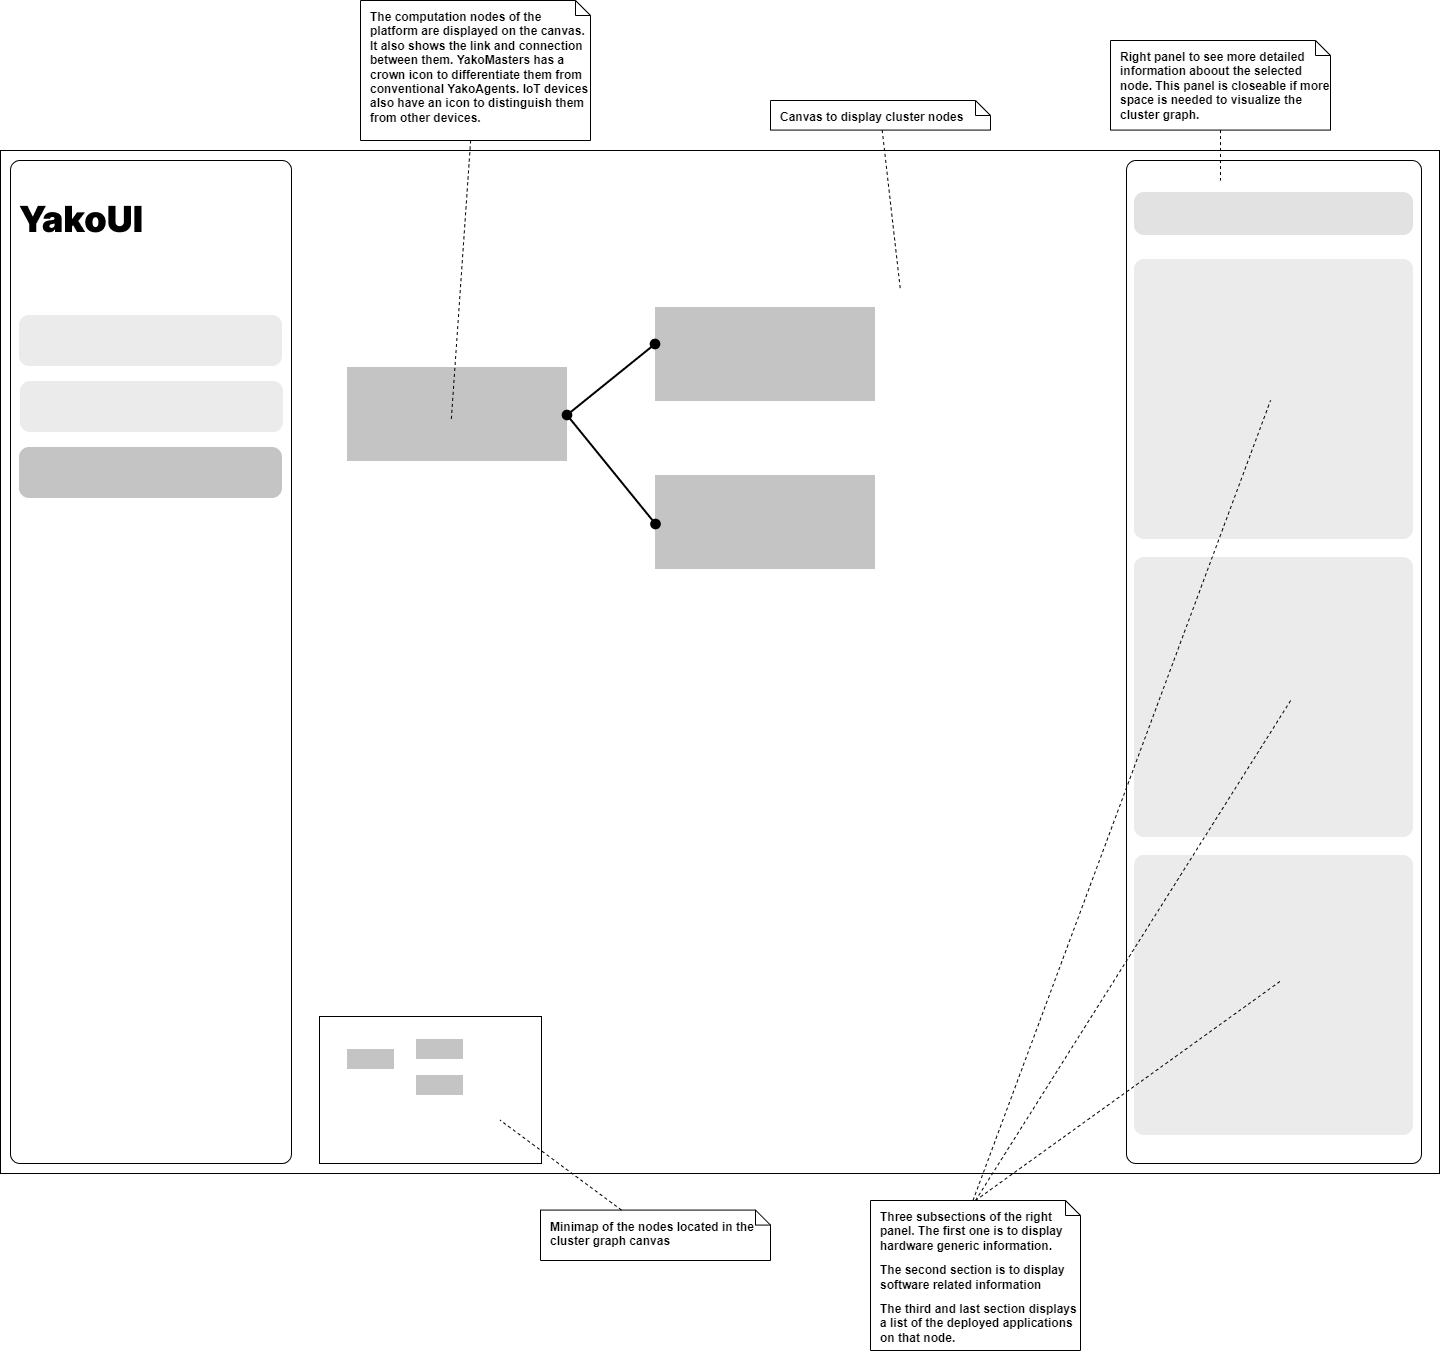
\includegraphics[width=0.8\linewidth]{/Frontend/YakoUI cluster graph wireframe.png}
                    \caption{YakoUI cluster graph wireframe}
                    \label{fig:cluster_wireframe}
                \end{figure}
                
            \subsubsubsubsection{Dashboard wireframe}
                This view tab is where all the information is gathered. The same nodes are shown in the left side of the page. On the top right side, a list of the top YakoAgent where the previously uploaded application could be uploaded are shown in descent order.
                The down right corner is reserved to display a list of the previously deployed application.
                
                \begin{figure}[H]
                    \centering
                    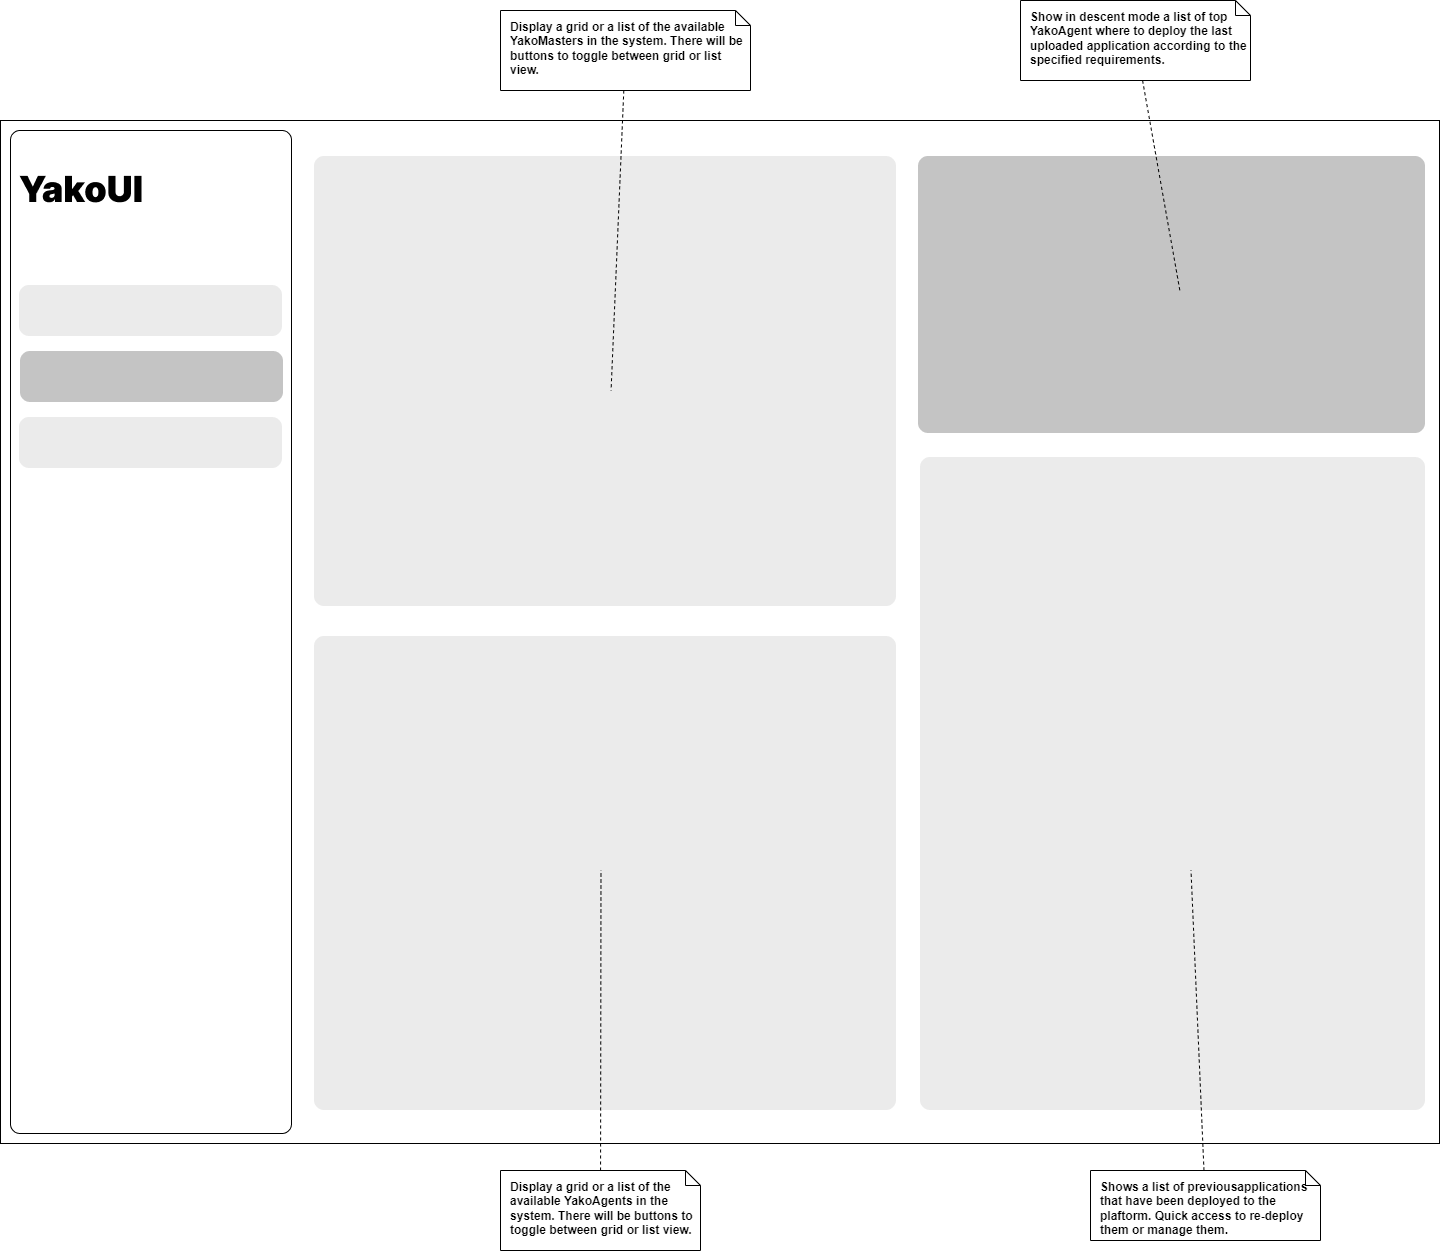
\includegraphics[width=0.8\linewidth]{/Frontend/YakoUI Dashboard wireframe.png}
                    \caption{YakoUI dashboard wireframe}
                    \label{fig:dashboard_wireframe}
                \end{figure}
                
            \subsubsubsubsection{Upload and Deploy application wireframe}
                This view tab is the entry point of the platform. It will be shown on application start up, a drag and drop area is shown in the center where the system administrator could select the application to be deployed in the system.
                
                \begin{figure}[H]
                    \centering
                    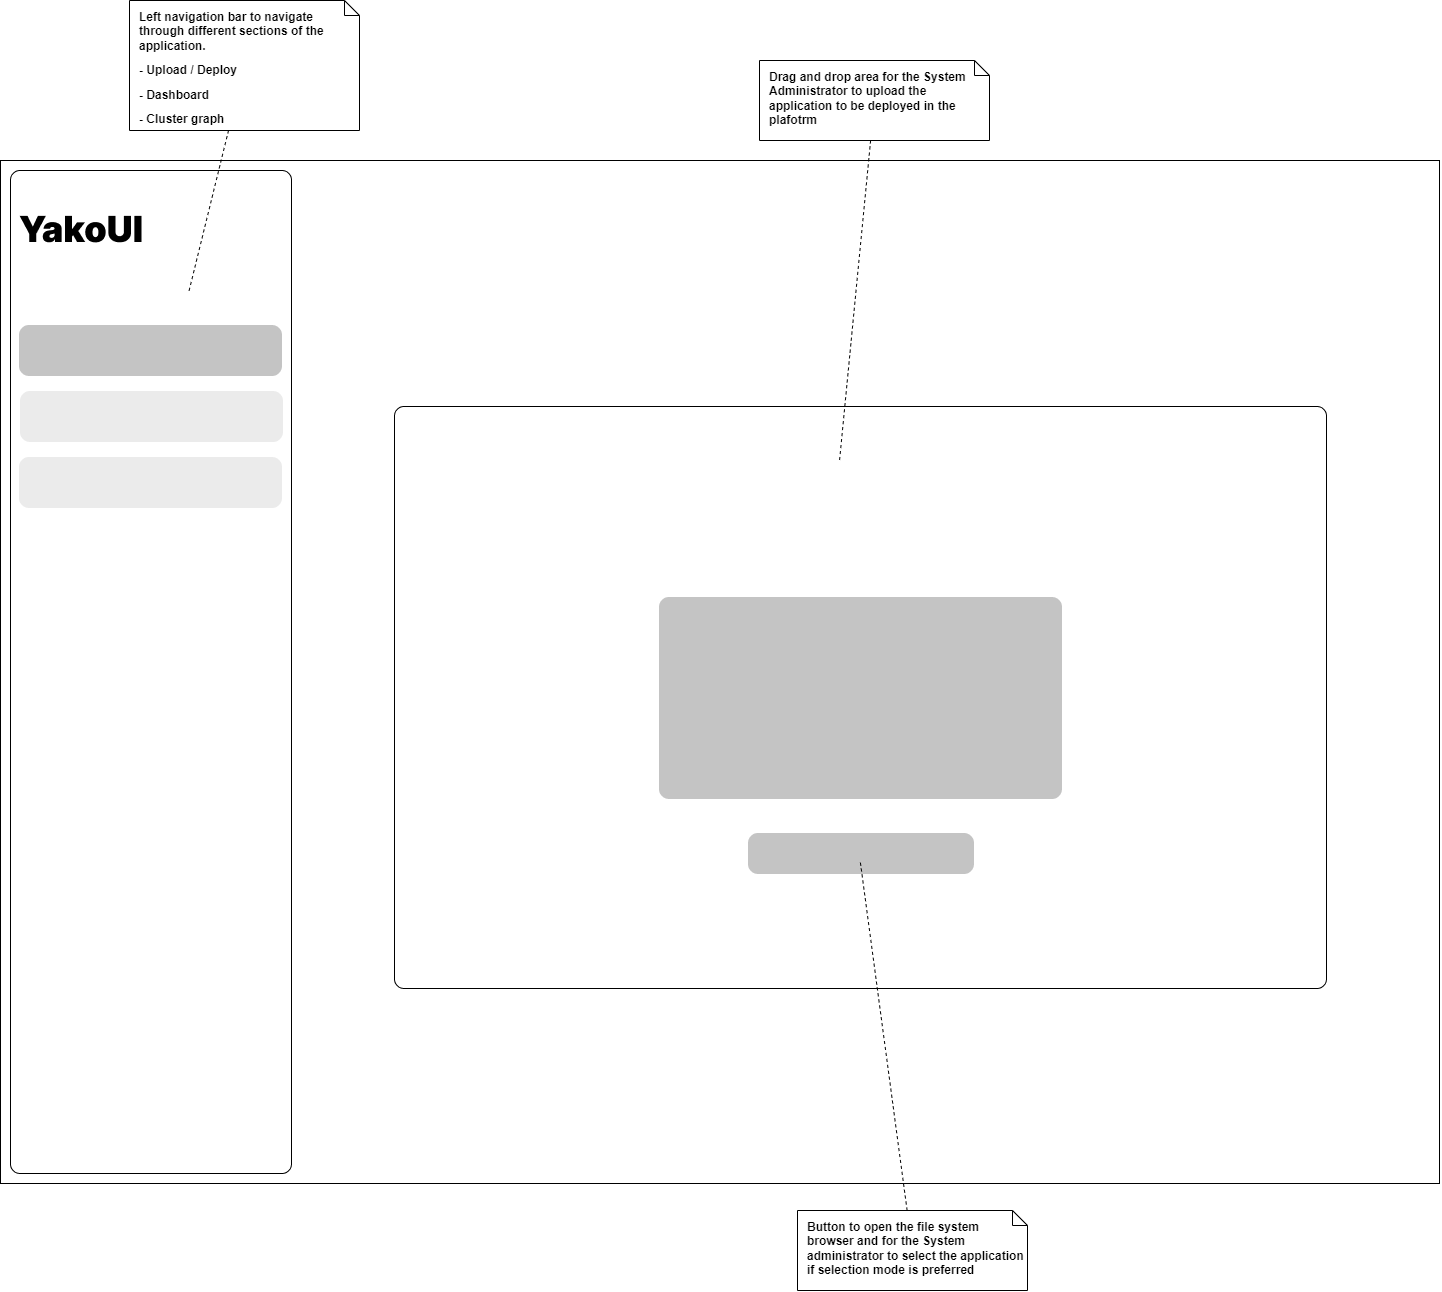
\includegraphics[width=0.8\linewidth]{/Frontend/YakoUI deploy app wireframe.png}
                    \caption{YakoUI deploy app wireframe}
                    \label{fig:deploy_wireframe}
                \end{figure}
        
        \subsubsubsection{Stage 2: UI prototyping}
            In this second stage, all the previous low-fidelity wireframes were converted into UI prototypes. These includes more details on the sections. In this step a design system was defined.
            
            \subsubsubsubsection{Dashboard User Interface}
                The dashboard page provides a visual display of the platform. The view is divided horizontally in two sections, on the left side there are two subsections where the information about all the agents including the YakoMasters are displayed. For usability purpose, located on the top right corner of these sections two views styles buttons, grid and list, have been provided. Toggling between them will change the displaying format.
                
                On the other half of this page, two other sections are reserved to display Top Nodes and the list of uploaded Applications. The node cards should display the agent identifier and the resources that comply with the requested system resources are highlighted in green, while those that do not fulfil are marked in red.
                
                The enumerations of the Applications section are presented as a list of application cards. These cards show the application name on the left side, and buttons to interact with these are situated on the other side.
                \begin{figure}[H]
                    \centering
                    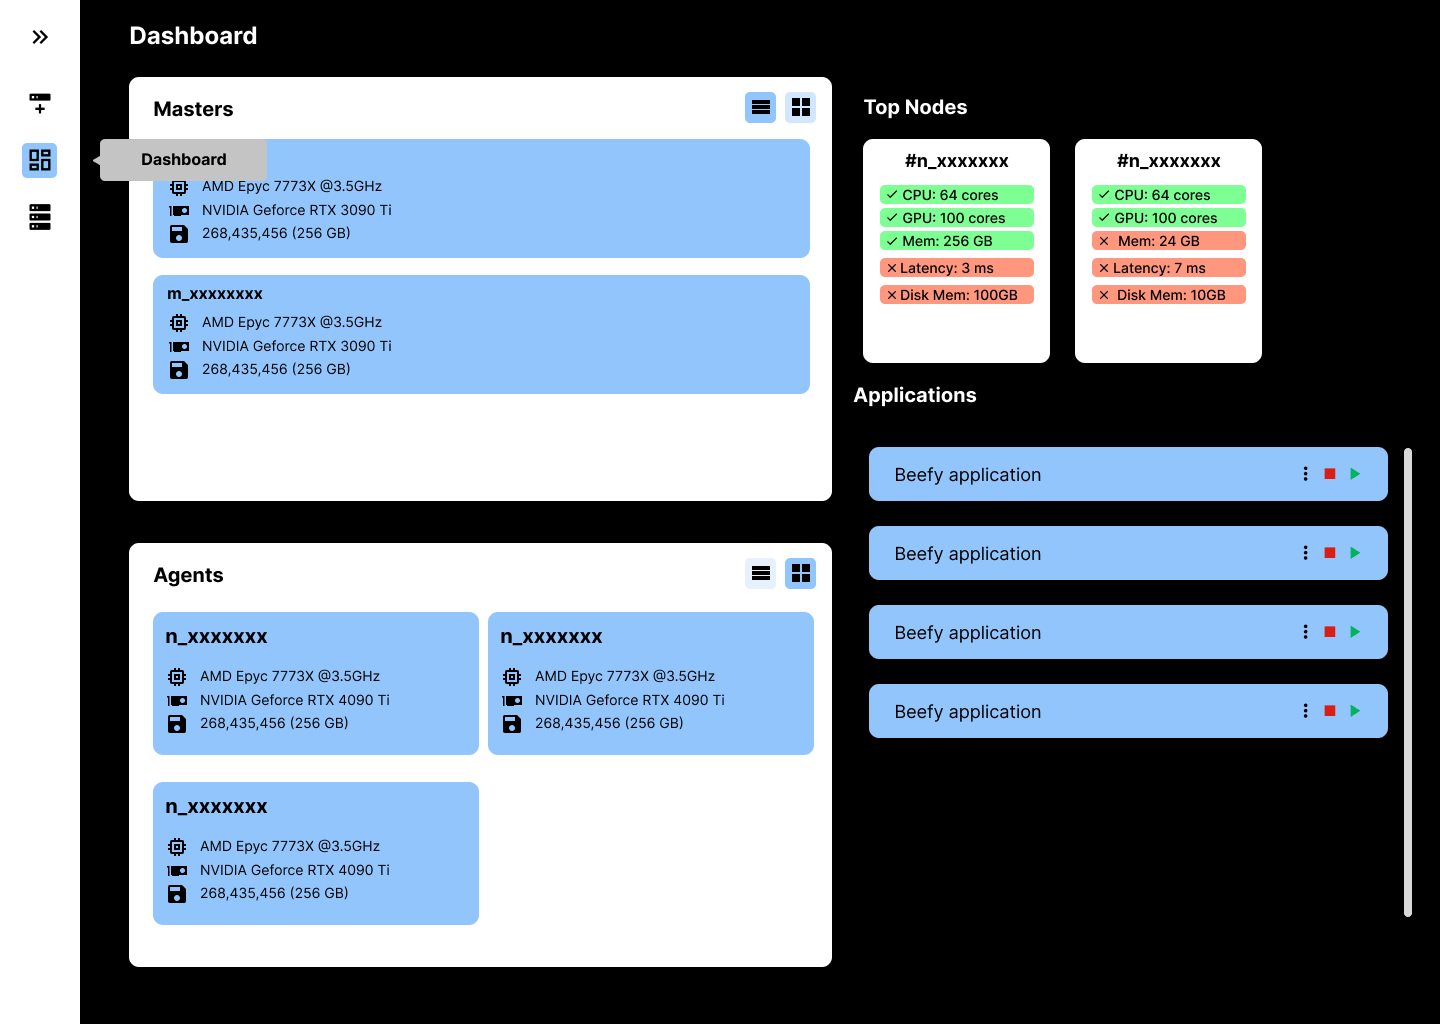
\includegraphics[width=\linewidth]{Images/Frontend/UI/YakoUI Dashboard UI.png}
                    \caption{YakoUI dashboard UI}
                    \label{fig:dashboard_ui}
                \end{figure}
            
            \subsubsubsubsection{Cluster graph User Interface}
                The Cluster Graph page shows available nodes in a graphical mode. An extended version of the data is situated in the right side. It can be displayed at user's convenience by clicking on any of the nodes. This panel is divided into 4 main sections, General Information, System Information, Network Information and Deployed Applications lists shows the active running applications on that node.
                
                An even more detailed version of the previously expanded right panel, figure \ref{fig:expanded_info_panel_ui},  can be shown by clicking the left chevron tab situated in the left center part. On click it will enlarge the floating window showing the same amount of previous information with the addition of several graphs and telemetry in graphical mode.
            
                \begin{figure}[H]
                    \centering
                    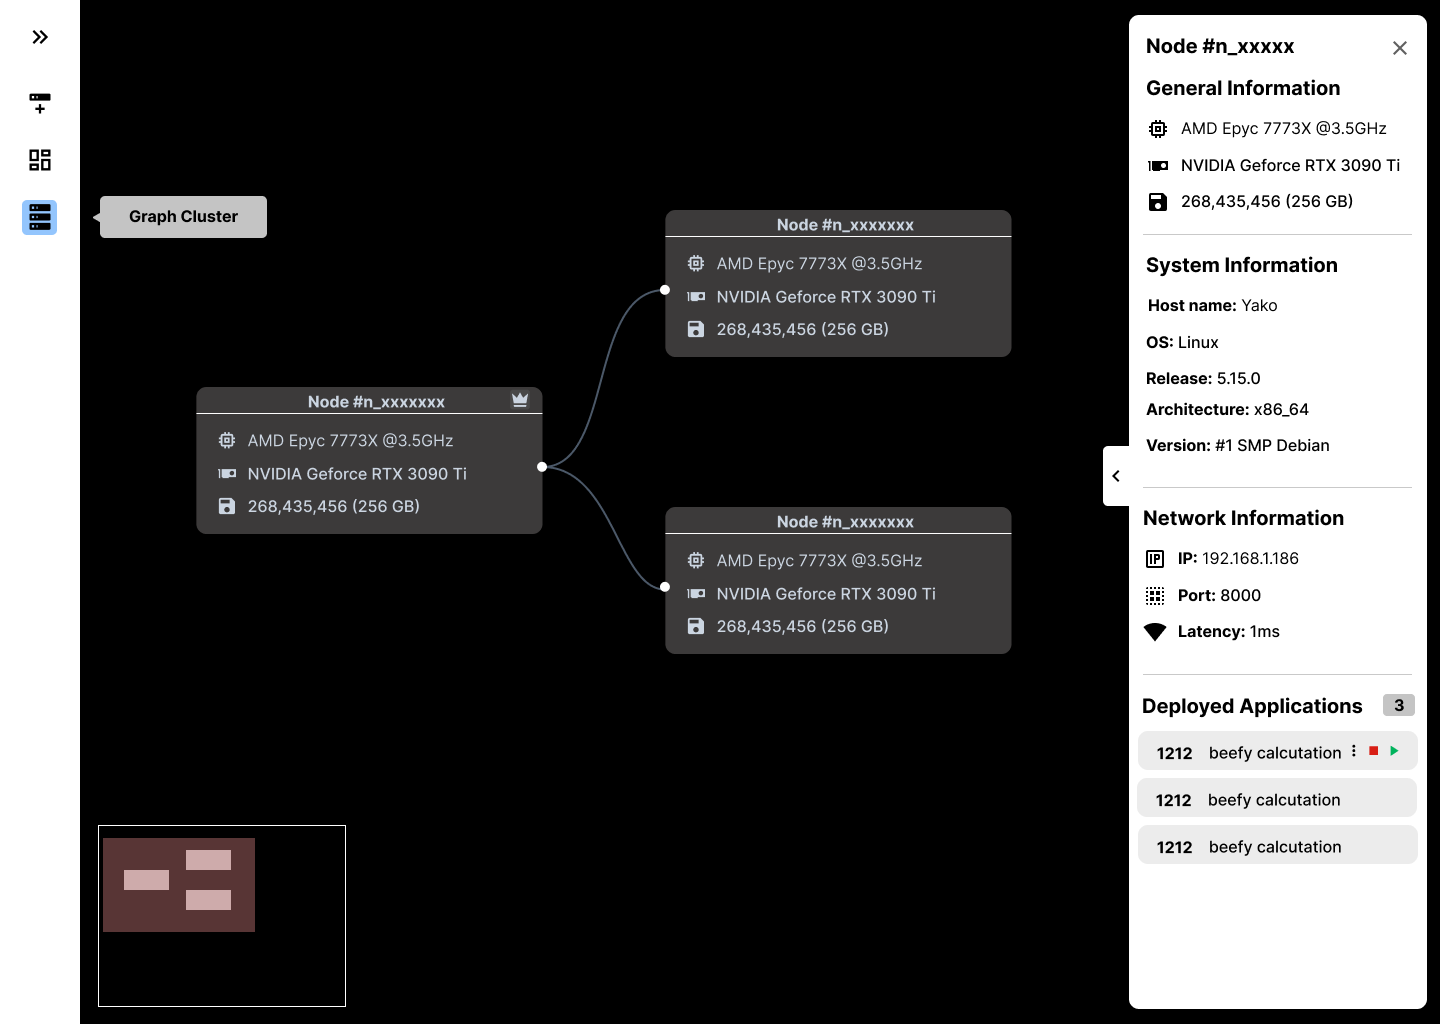
\includegraphics[width=0.85\linewidth]{Images/Frontend/UI/YakoUI Graph Cluster UI.png}
                    \caption{YakoUI Cluster Graph UI}
                    \label{fig:cluster_graph_ui}
                \end{figure}
                
                This view, figure \ref{fig:expanded_info_panel_ui},  was not developed for the delivered v1 software, due to time constraints and the prioritization of other major features.
                
                \begin{figure}[H]
                    \centering
                    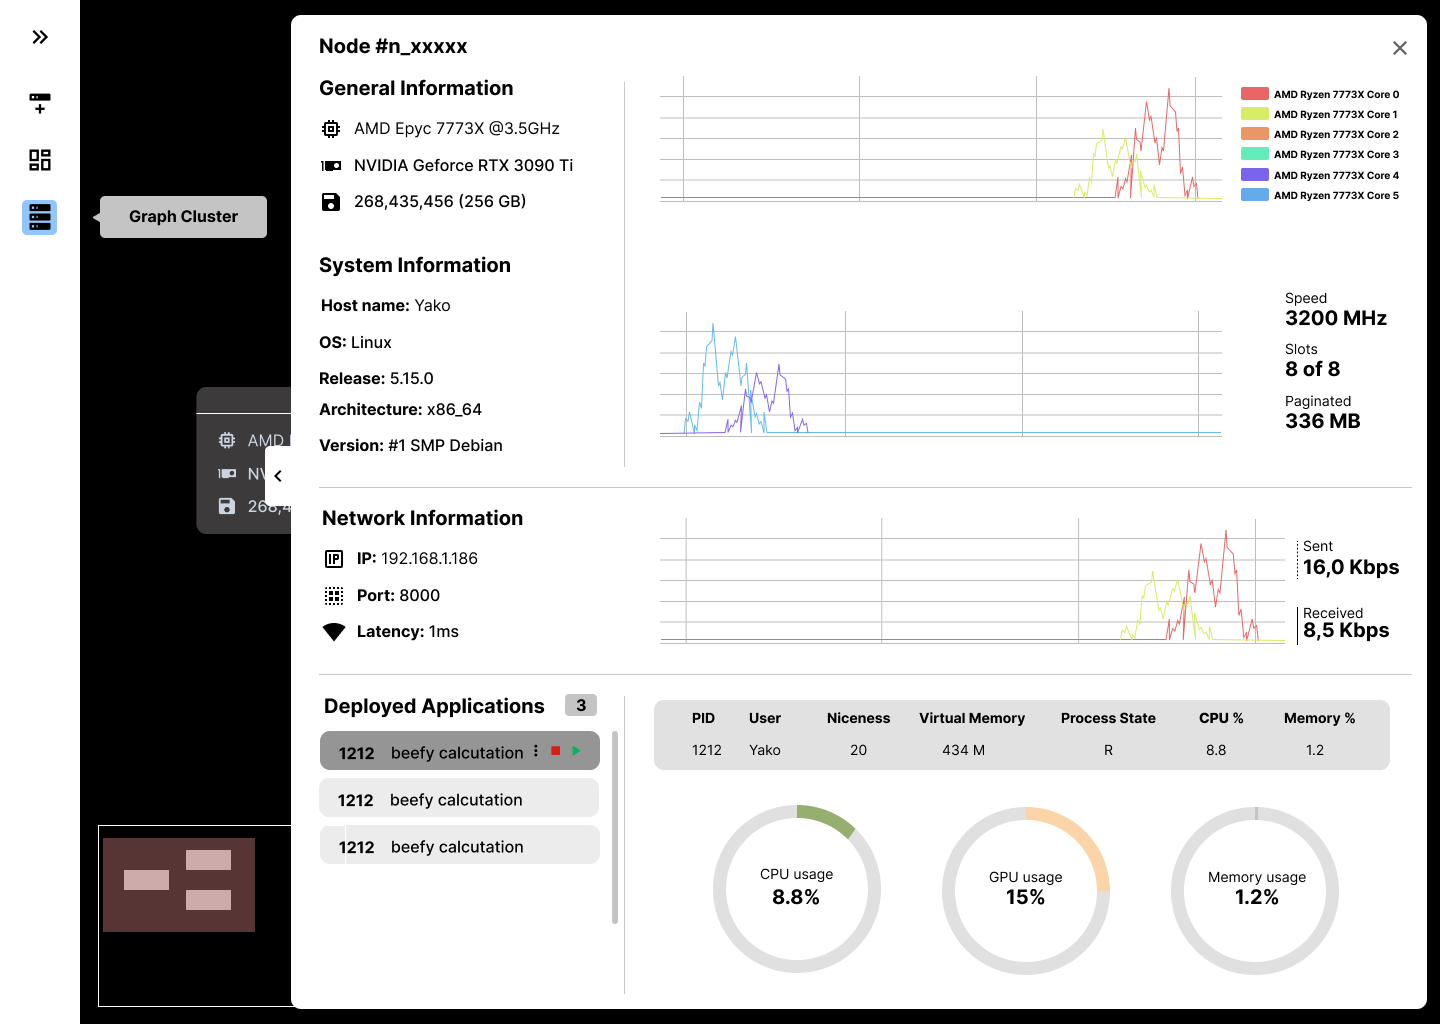
\includegraphics[width=0.85\linewidth]{Images/Frontend/UI/YakoUI Expanded YakoAgent Information Panel UI.png}
                    \caption{YakoUI Expanded YakoAgent Information Panel UI}
                    \label{fig:expanded_info_panel_ui}
                \end{figure}
            
            \subsubsubsubsection{Upload and Deploy application User Interface}
                This is the first page that will be presented to the user on application start up. This view consists of a region where the system administrator can drag and drop the application to be deployed in the cluster. If manual selection is preferred, a "Select file" button is made available.
                
                \begin{figure}[H]
                    \centering
                    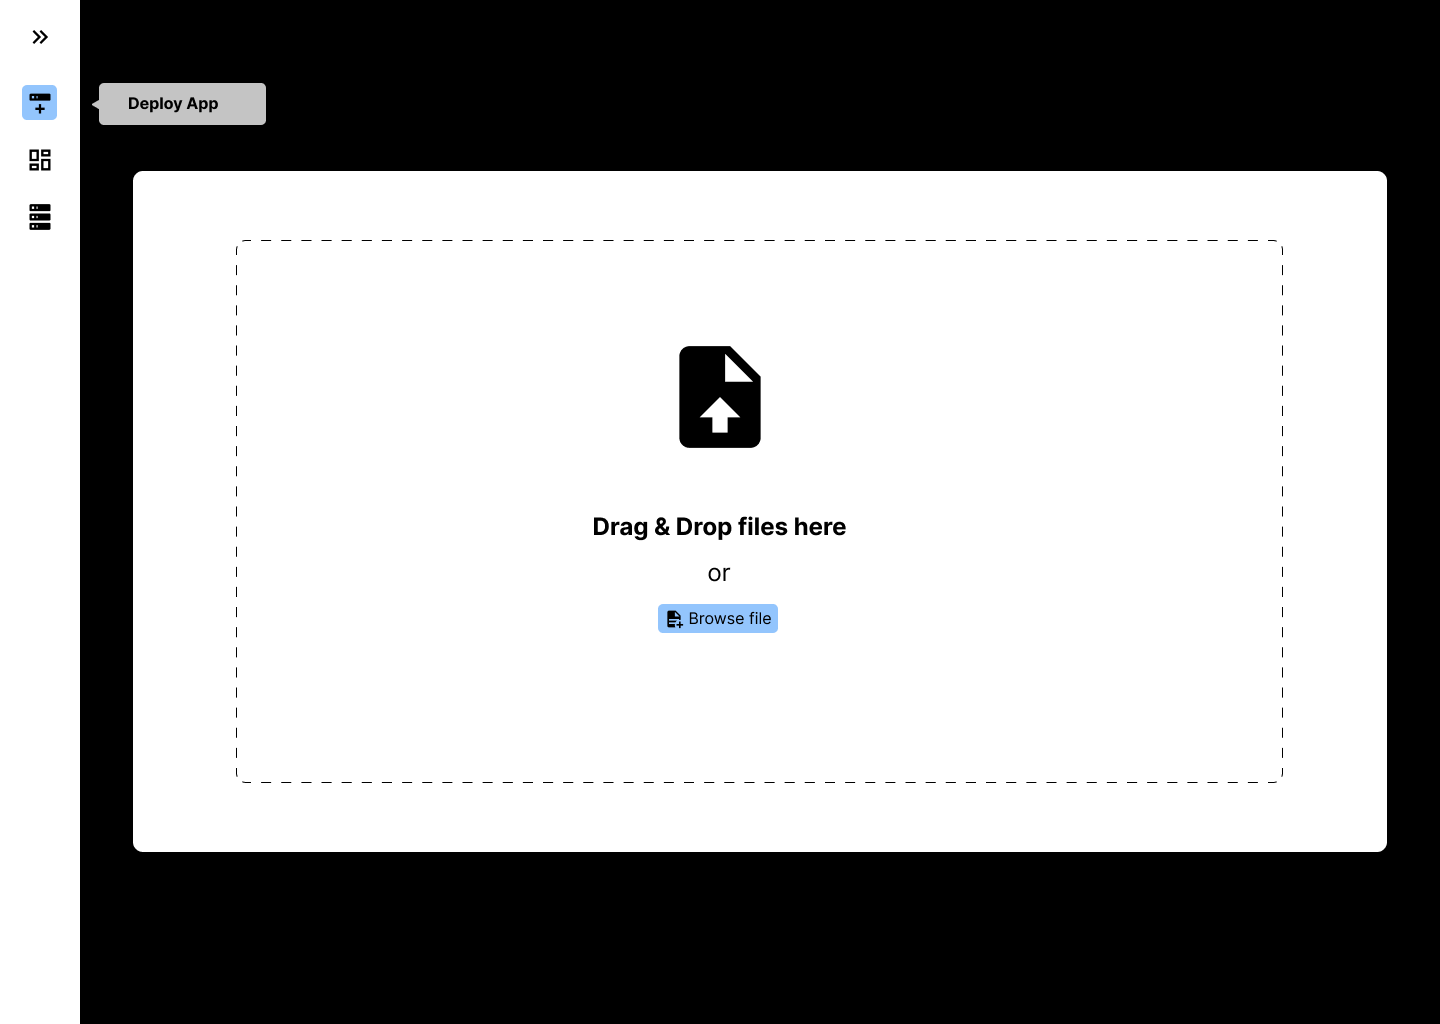
\includegraphics[width=0.7\linewidth]{Images/Frontend/UI/YakoUI Upload Application UI.png}
                    \caption{YakoUI Deploy Application UI}
                    \label{fig:deploy_app_ui}
                \end{figure}
            
                Once the application has been selected, a pop-up form will appear, figure \ref{fig:upload_form}.
                
                \begin{figure}[H]
                \centering
                    \begin{subfigure}{0.45\textwidth}
                        \centering
                        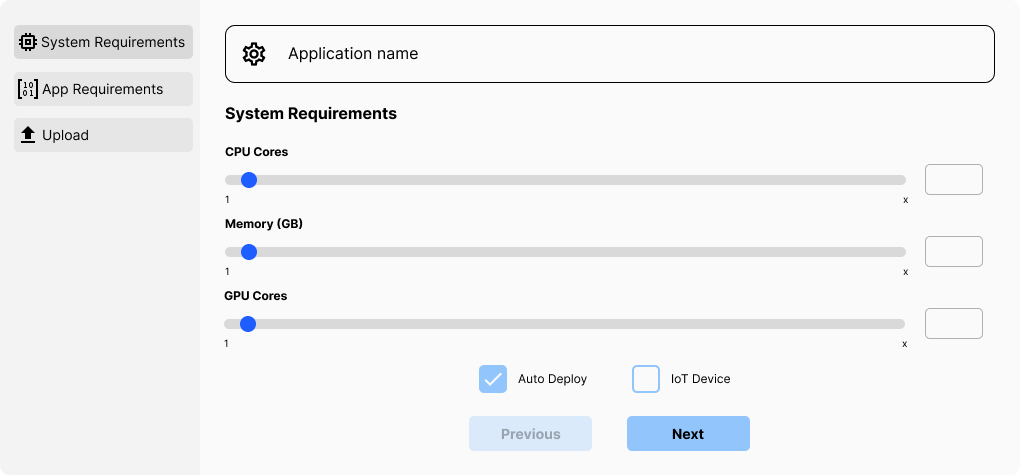
\includegraphics[width=\textwidth]{Images/Frontend/UI/YakoUI Form 1.png}
                        \subcaption{System Requirements form}
                        \label{fig:form_1}
                    \end{subfigure}
                    \begin{subfigure}{0.45\textwidth}
                        \centering
                        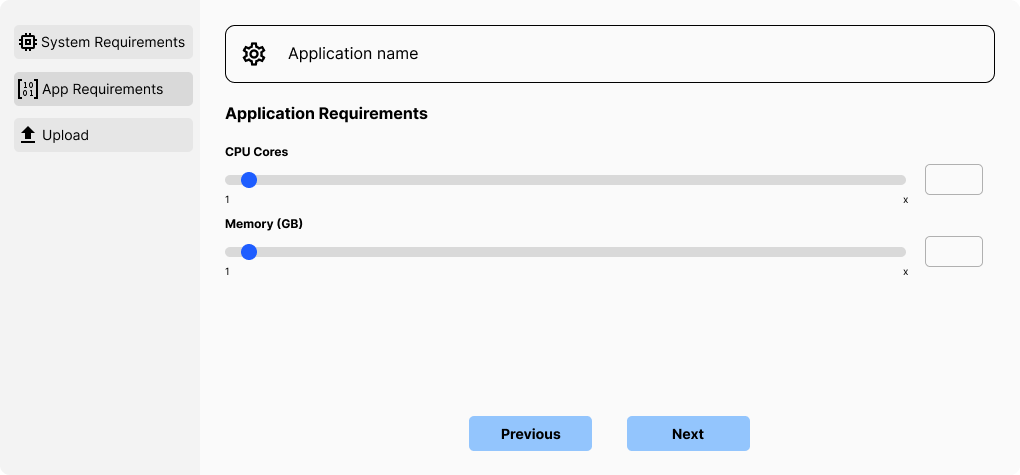
\includegraphics[width=\textwidth]{Images/Frontend/UI/YakoUI Form 2.png}
                        \subcaption{Application Requirements form}
                        \label{fig:form_2}
                    \end{subfigure}
                    \vskip\baselineskip
                    \begin{subfigure}{\textwidth}
                        \centering
                        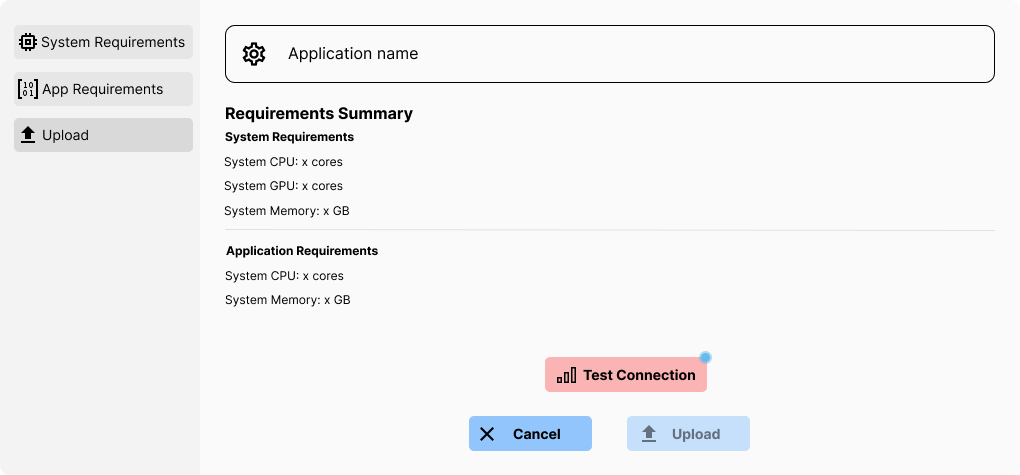
\includegraphics[width=0.45\textwidth]{Images/Frontend/UI/YakoUI Form 3.png}
                        \subcaption{Summary form tab}
                        \label{fig:form_3}
                    \end{subfigure}
                    \caption{Upload application form}
                    \label{fig:upload_form}
                \end{figure}
                
                This window contains 3 tabs. The first asks the user to select all the preferred specifications of the system where the binary will be ran. These system requirements specifications will be collected to find the most suitable node of the cluster.
                The following tab collects resources for the virtualization of the application (The back-end logic for this feature could not been developed for release v1).
                The last tab summarizes all the selected properties. A connection test must be fired before being able to upload and deploy the application.
    
    \subsection{Run the system}
    
        This section describes the steps to run the Yako platform, both back-end and front-end software.
        
        % Steps to run the entire system
        \subsubsection{Run the back-end}

    \subsubsubsection{Dependencies}
        Before being able to compile YakoMaster, YakoAgent and YakoAgent (IoT), projects tools and dependencies must be installed in the system. All three applications are programmed in Golang, Google's open-sourced programming language.
        
        The following enumeration lists all the tools required to compile the platform.
    
        \begin{enumerate}
            \item \href{https://go.dev/dl/}{Golang v1.17.x or greater}
            \item \href{https://www.gnu.org/software/make/}{Make}
            \item \href{https://zookeeper.apache.org/releases.html}{Apache Zookeeper}
            \item \href{https://grpc.io/docs/languages/go/quickstart/}{gRPC}
            \item \href{https://developers.google.com/protocol-buffers}{Protocol buffers compiler (Protobuf)}
            \item \href{https://mosquitto.org/download/}{Eclipse Mosquitto MQTT Broker}
        \end{enumerate}

    \subsubsubsection{Compilation}
        A Makefile is available in the source code repository. Table \ref{tab:yako_make} lists all the predefined make rules. 

        \begin{table}[H]
            \centering
            \caption{Makefile rules for make}
            \begin{tabularx}{\linewidth}{|l|>{\raggedright}p{70mm}|X|}
            \hline
            \rowcolor[HTML]{C0C0C0}
            \textbf{Rule} & \textbf{Script} & \textbf{Description} \\ \hline
            gen\_proto & protoc --proto\_path=src/grpc/proto/ --go-grpc\_opt = require\_unimplemented\_servers = false --go\_out=src/grpc/ --go-grpc\_out=src/grpc/ src/grpc/proto/\*.proto & Generates the protobufs code used by the gRPC client \& server from the .proto source code \\ \hline
            
            clean & rm src/grpc/pb/*.go & Cleans the generated protobuf files \\ \hline
            
            build\_master & go build src/yako\_master/YakoMaster.go & Compiles YakoMaster \\ \hline
            
            run\_master & ./src/yako\_master/YakoMaster \$(ip) \$(port) \$(zk\_ip) \$(zk\_port) \$(mqtt\_ip) \$(mqtt\_port) & Runs the YakoMaster \\ \hline
            
            build\_agent & go build src/yako\_node/YakoAgent.go & Compiles YakoAgent \\ \hline
            
            run\_agent & ./src/yako\_node/YakoAgent \$(ip) \$(port) \$(zk\_ip) \$(zk\_port) & Runs the YakoAgent \\ \hline
            
            build\_agent\_iot & go build src/yako\_agent\_iot/YakoAgentIoT.go & Compiles YakoAgent (IoT) \\ \hline
            
            run\_agent\_iot & ./src/yako\_agent\_iot/YakoAgentIoT \$(ip) \$(port) \$(mqtt\_ip) \$(mqtt\_port) & Runs the YakoMaster (IoT) \\ \hline
            \end{tabularx}
            \label{tab:yako_make}
        \end{table}
        
        \subsubsubsubsection{gRPC and Protocol Buffers}
            gRPC stubs and procedures must be generated before proceeding with the project setup.
            Ensure that the system have these Go plugins installed, used for protocol buffers' compilation. This includes Golang gRPC and Golang Protocol Buffers compiler. Generate the Go gRPC source code by executing running the following code snippet.

            \begin{code}
                \inputminted[
                    frame=lines,
                    framesep=2mm,
                    baselinestretch=1,
                    bgcolor=LightGray,
                    fontsize=\footnotesize,
                    breaklines=true,
                    linenos
                ]{bash}{Code/Deploy/install_grpc_deps.sh}
                \caption{Golang gRPC dependencies Installation}
                \label{code:install_grpc_deps}
            \end{code}
            
            Yako platform software dependencies are located in the modules file go.mod, these must be installed first. Download these using snippet \ref{code:mod_tidy}. Finally, to build all three programs run code snippet \ref{code:compile}.
            
            \begin{code}
                \inputminted[
                    frame=lines,
                    framesep=2mm,
                    baselinestretch=1,
                    bgcolor=LightGray,
                    fontsize=\footnotesize,
                    breaklines=true,
                    linenos
                ]{bash}{Code/Deploy/mod_tidy.sh}
                \caption{Download and install Golang Dependencies}
                \label{code:mod_tidy} 
            \end{code}

            \begin{code}
                \inputminted[
                    frame=lines,
                    framesep=2mm,
                    baselinestretch=1,
                    bgcolor=LightGray,
                    fontsize=\footnotesize,
                    breaklines=true,
                    linenos
                ]{bash}{Code/Deploy/compile.sh}
                \caption{Yako platform compilation}
                \label{code:compile} 
            \end{code}
        
    \subsubsubsection{Execution}
        Before running the Yako platform software, ZK and the Mosquitto MQTT broker must be fired up first. 
        \subsubsubsubsection{Zookeeper}
            To start or stop ZK, one must access the directory where Apache Zookeeper has been installed. Otherwise, if the binaries are loaded into the system PATH running code snippet \ref{code:run_zk} will do the work.
            
            \begin{code}
                \inputminted[
                    frame=lines,
                    framesep=2mm,
                    baselinestretch=1,
                    bgcolor=LightGray,
                    fontsize=\footnotesize,
                    breaklines=true,
                    linenos
                ]{bash}{Code/Deploy/run_zk.sh}
                \caption{Start/Stop Apache Zookeeper}
                \label{code:run_zk} 
            \end{code}
            
            The ZK configuration, zoo.cfg file, is stored in the /conf directory relative to the installed ZK path. To monitor and troubleshoot ZK, the provided Java client or C binary can be used.
            An example of the configuration file  \ref{code:zoo_conf} can be found in the project at Yako/src/utils/zookeeper/zoo.cnf. The highlighted line of code \ref{code:zoo_conf} should be replaced for the local ZK installation logs folder or a preferred custom path. In this configuration ZK also fires an administrator panel up at port 8081, it can be accessed with a browser on <zk\_ip>:8081/commands.

            \begin{code}
                \inputminted[
                    frame=lines,
                    framesep=2mm,
                    baselinestretch=1,
                    bgcolor=LightGray,
                    fontsize=\footnotesize,
                    escapeinside=||,
                    breaklines=true,
                    linenos
                ]{apacheconf}{Code/Deploy/zoo.cfg}
                \caption{Apache Zookeeper Configuration file}
                \label{code:zoo_conf}
            \end{code}

        \subsubsubsubsection{Mosquitto MQTT Broker}
            A configuration file is provided in the source code. The Mosquitto configuration file will set the broker to listen to the specified port, in the example below it starts the service at port 8002. For testing purposes, the broker also allows unauthenticated clients, Disable this property is recommended in production environment for security reasons. More specific documentation of Mosquitto broker can be found at its \textbf{\href{https://mosquitto.org/man/mosquitto-conf-5.html}{official website}}.

            \begin{code}
                \inputminted[
                    frame=lines,
                    framesep=2mm,
                    baselinestretch=1,
                    bgcolor=LightGray,
                    fontsize=\footnotesize,
                    breaklines=true,
                    linenos
                ]{apacheconf}{Code/Deploy/mosquitto.conf}
                \caption{Mosquitto MQTT Configuration file}
                \label{code:moquitto_conf}
            \end{code}

            Run the following command to start the MQTT broker. Appending a \& sign at the end makes the command run in the background.
            
            \begin{code}
                \inputminted[
                    frame=lines,
                    framesep=2mm,
                    baselinestretch=1,
                    bgcolor=LightGray,
                    fontsize=\footnotesize,
                    breaklines=true,
                    linenos
                ]{bash}{Code/Deploy/run_mosquitto.sh}
                \caption{Start Mosquitto MQTT broker}
                \label{code:run_mosquitto}
            \end{code}

        \subsubsubsubsection{YakoMaster}
            YakoMaster accepts a total of six arguments. The first two arguments, firstly the IP and secondly the port, are used to specify the socket of the machine where it will be run. The next two arguments are used to specify the socket of the ZK service registry machine that could be located in a separate physical machine. The final two arguments are needed to specify the location of the Mosquitto MQTT Broker.
    
            - Make rule:
            
            \begin{code}
                \inputminted[
                    frame=lines,
                    framesep=2mm,
                    baselinestretch=1,
                    bgcolor=LightGray,
                    fontsize=\footnotesize,
                    breaklines=true,
                    linenos
                ]{bash}{Code/Deploy/yakomaster_deploy_make.sh}
                \caption{YakoMaster make rule}
                \label{code:yakomaster_deploy_make}
            \end{code}
            
            - Manual deploy:
            
            \begin{code}
                \inputminted[
                    frame=lines,
                    framesep=2mm,
                    baselinestretch=1,
                    bgcolor=LightGray,
                    fontsize=\footnotesize,
                    breaklines=true,
                    linenos
                ]{bash}{Code/Deploy/yakomaster_deploy.sh}
                \caption{YakoMaster manual deploy}
                \label{code:yakomaster_deploy}
            \end{code}

        \subsubsubsubsection{YakoAgent}
            To deploy a YakoAgent, four arguments must be passed, the first two are the agent's machine IP and Port, while the last two are the location of the service registry. On connection, YakoMaster will be automatically notified.
            
            - Make rule:
            
            \begin{code}
                \inputminted[
                    frame=lines,
                    framesep=2mm,
                    baselinestretch=1,
                    bgcolor=LightGray,
                    fontsize=\footnotesize,
                    breaklines=true,
                    linenos
                ]{bash}{Code/Deploy/yakoagent_deploy_make.sh}
                \caption{YakoAgent make rule}
                \label{code:yakoagent_deploy_make}
            \end{code}
            
            - Manual deploy:
                
            \begin{code}
                \inputminted[
                    frame=lines,
                    framesep=2mm,
                    baselinestretch=1,
                    bgcolor=LightGray,
                    fontsize=\footnotesize,
                    breaklines=true,
                    linenos
                ]{bash}{Code/Deploy/yakoagent_deploy.sh}
                \caption{YakoAgent manual deploy}
                \label{code:yakoagent_deploy}
            \end{code}
        
        \subsubsubsubsection{YakoAgent (IoT)}
            To deploy a YakoAgent (IoT), four arguments must be assigned, the device's location and the Mosquitto MQTT broker socket.
            
            - Make rule:
            
            \begin{code}
                \inputminted[
                    frame=lines,
                    framesep=2mm,
                    baselinestretch=1,
                    bgcolor=LightGray,
                    fontsize=\footnotesize,
                    breaklines=true,
                    linenos
                ]{bash}{Code/Deploy/yakoagentiot_deploy_make.sh}
                \caption{YakoAgent (IoT) make rule}
                \label{code:yakoagentiot_deploy_make}
            \end{code}
            
            - Manual deploy:
            
            \begin{code}
                \inputminted[
                    frame=lines,
                    framesep=2mm,
                    baselinestretch=1,
                    bgcolor=LightGray,
                    fontsize=\footnotesize,
                    breaklines=true,
                    linenos
                ]{bash}{Code/Deploy/yakoagentiot_deploy.sh}
                \caption{YakoAgent (IoT) manual deploy}
                \label{code:yakoagentiot_deploy}
            \end{code}

        \subsubsection{Run the front-end}
    \subsubsubsection{Dependencies}
        Firstly, ensure that the following two tools are installed in the system. The installation of NPM is generally bundled into NodeJS.
        
        \begin{enumerate}
            \item \href{https://nodejs.org/en/}{NodeJS}
            \item \href{https://www.npmjs.com/package/npm}{Node Package Manager (NPM)}
        \end{enumerate}
        
    \subsubsubsection{Compilation}
        The front-end application's dependencies and other meta-data are located into the package.json. Firstly, installing these libraries is required. Secondly, table \ref{tab:npm_scripts} lists all pre-defined commands to build the application.
        
        \begin{code}
            \inputminted[
                frame=lines,
                framesep=2mm,
                baselinestretch=1,
                bgcolor=LightGray,
                fontsize=\footnotesize,
                breaklines=true,
                linenos
            ]{bash}{Code/Deploy/npm_install.sh}
            \caption{Install project dependencies}
            \label{code:npm_install}
        \end{code}
        
        \begin{table}[H]
            \centering
            \caption{NPM scripts in package.json}
            \begin{tabularx}{\linewidth}{|l|>{\raggedright}p{70mm}|X|}
            \hline
            \rowcolor[HTML]{C0C0C0}
            \textbf{Rule} & \textbf{Script} & \textbf{Description} \\ \hline
            serve & vue-cli-service serve & Starts a development server served on the browser \\ \hline
            build & vue-cli-service build & Builds application to be served on the browser \\ \hline
            lint & vue-cli-service lint & Analyse code for potential errors \\ \hline
            electron:serve & vue-cli-service electron:serve & Starts a development application server \\ \hline
            build-win & vue-cli-service electron:build --win --ia32 --x64 --publish=onTagOrDraft & Builds the desktop application for Windows OS 32-bits and 64-bits architecture \\ \hline
            build-mac & vue-cli-service electron:build --mac --publish=onTagOrDraft" & Builds the desktop application for macOS \\ \hline
            build-linux & vue-cli-service electron:build --linux --publish=onTagOrDraft & Builds the desktop application for Linux \\ \hline
            \end{tabularx}
            \label{tab:npm_scripts}
        \end{table}
    
        For Windows OS systems, the application can be compiled as an installer or a portable executable for both 32-bits and 64-bits architecture systems. For MacOS, the bundled application is both instalable and portable. For Linux based system, different installers for different Linux distributions are generated. Please refer to the specific OS flavour official manual to install its packages.
